\documentclass[conference,compsoc]{IEEEtran}
\newcommand{\bsptitle}{Google Cloud Platform}

\usepackage{xcolor}
\usepackage{graphicx}
	
\usepackage{datetime}

% *** CITATION PACKAGES ***
%
\ifCLASSOPTIONcompsoc
% IEEE Computer Society needs nocompress option
% requires cite.sty v4.0 or later (November 2003)
\usepackage[nocompress]{cite}
\else
% normal IEEE
\usepackage{cite}
\fi
% cite.sty was written by Donald Arseneau
% V1.6 and later of IEEEtran pre-defines the format of the cite.sty package
% \cite{} output to follow that of the IEEE. Loading the cite package will
% result in citation numbers being automatically sorted and properly
% "compressed/ranged". e.g., [1], [9], [2], [7], [5], [6] without using
% cite.sty will become [1], [2], [5]--[7], [9] using cite.sty. cite.sty's
% \cite will automatically add leading space, if needed. Use cite.sty's
% noadjust option (cite.sty V3.8 and later) if you want to turn this off
% such as if a citation ever needs to be enclosed in parenthesis.
% cite.sty is already installed on most LaTeX systems. Be sure and use
% version 5.0 (2009-03-20) and later if using hyperref.sty.
% The latest version can be obtained at:
% http://www.ctan.org/pkg/cite
% The documentation is contained in the cite.sty file itself.
%
% Note that some packages require special options to format as the Computer
% Society requires. In particular, Computer Society  papers do not use
% compressed citation ranges as is done in typical IEEE papers
% (e.g., [1]-[4]). Instead, they list every citation separately in order
% (e.g., [1], [2], [3], [4]). To get the latter we need to load the cite
% package with the nocompress option which is supported by cite.sty v4.0
% and later.

% *** GRAPHICS RELATED PACKAGES ***
%
\ifCLASSINFOpdf
% \usepackage[pdftex]{graphicx}
% declare the path(s) where your graphic files are
% \graphicspath{{../pdf/}{../jpeg/}}
% and their extensions so you won't have to specify these with
% every instance of \includegraphics
% \DeclareGraphicsExtensions{.pdf,.jpeg,.png}
\else
% or other class option (dvipsone, dvipdf, if not using dvips). graphicx
% will default to the driver specified in the system graphics.cfg if no
% driver is specified.
% \usepackage[dvips]{graphicx}
% declare the path(s) where your graphic files are
% \graphicspath{{../eps/}}
% and their extensions so you won't have to specify these with
% every instance of \includegraphics
% \DeclareGraphicsExtensions{.eps}
\fi
% graphicx was written by David Carlisle and Sebastian Rahtz. It is
% required if you want graphics, photos, etc. graphicx.sty is already
% installed on most LaTeX systems. The latest version and documentation
% can be obtained at: 
% http://www.ctan.org/pkg/graphicx
% Another good source of documentation is "Using Imported Graphics in
% LaTeX2e" by Keith Reckdahl which can be found at:
% http://www.ctan.org/pkg/epslatex
%
% latex, and pdflatex in dvi mode, support graphics in encapsulated
% postscript (.eps) format. pdflatex in pdf mode supports graphics
% in .pdf, .jpeg, .png and .mps (metapost) formats. Users should ensure
% that all non-photo figures use a vector format (.eps, .pdf, .mps) and
% not a bitmapped formats (.jpeg, .png). The IEEE frowns on bitmapped formats
% which can result in "jaggedy"/blurry rendering of lines and letters as
% well as large increases in file sizes.
%
% You can find documentation about the pdfTeX application at:
% http://www.tug.org/applications/pdftex


% *** MATH PACKAGES ***
%
%\usepackage{amsmath}
% A popular package from the American Mathematical Society that provides
% many useful and powerful commands for dealing with mathematics.
%
% Note that the amsmath package sets \interdisplaylinepenalty to 10000
% thus preventing page breaks from occurring within multiline equations. Use:
%\interdisplaylinepenalty=2500
% after loading amsmath to restore such page breaks as IEEEtran.cls normally
% does. amsmath.sty is already installed on most LaTeX systems. The latest
% version and documentation can be obtained at:
% http://www.ctan.org/pkg/amsmath

% *** SPECIALIZED LIST PACKAGES ***
%
%\usepackage{algorithmic}
% algorithmic.sty was written by Peter Williams and Rogerio Brito.
% This package provides an algorithmic environment fo describing algorithms.
% You can use the algorithmic environment in-text or within a figure
% environment to provide for a floating algorithm. Do NOT use the algorithm
% floating environment provided by algorithm.sty (by the same authors) or
% algorithm2e.sty (by Christophe Fiorio) as the IEEE does not use dedicated
% algorithm float types and packages that provide these will not provide
% correct IEEE style captions. The latest version and documentation of
% algorithmic.sty can be obtained at:
% http://www.ctan.org/pkg/algorithms
% Also of interest may be the (relatively newer and more customizable)
% algorithmicx.sty package by Szasz Janos:
% http://www.ctan.org/pkg/algorithmicx


% *** ALIGNMENT PACKAGES ***
%
%\usepackage{array}
% Frank Mittelbach's and David Carlisle's array.sty patches and improves
% the standard LaTeX2e array and tabular environments to provide better
% appearance and additional user controls. As the default LaTeX2e table
% generation code is lacking to the point of almost being broken with
% respect to the quality of the end results, all users are strongly
% advised to use an enhanced (at the very least that provided by array.sty)
% set of table tools. array.sty is already installed on most systems. The
% latest version and documentation can be obtained at:
% http://www.ctan.org/pkg/array

% IEEEtran contains the IEEEeqnarray family of commands that can be used to
% generate multiline equations as well as matrices, tables, etc., of high
% quality.

% *** SUBFIGURE PACKAGES ***
%\ifCLASSOPTIONcompsoc
%  \usepackage[caption=false,font=footnotesize,labelfont=sf,textfont=sf]{subfig}
%\else
%  \usepackage[caption=false,font=footnotesize]{subfig}
%\fi
% subfig.sty, written by Steven Douglas Cochran, is the modern replacement
% for subfigure.sty, the latter of which is no longer maintained and is
% incompatible with some LaTeX packages including fixltx2e. However,
% subfig.sty requires and automatically loads Axel Sommerfeldt's caption.sty
% which will override IEEEtran.cls' handling of captions and this will result
% in non-IEEE style figure/table captions. To prevent this problem, be sure
% and invoke subfig.sty's "caption=false" package option (available since
% subfig.sty version 1.3, 2005/06/28) as this is will preserve IEEEtran.cls
% handling of captions.
% Note that the Computer Society format requires a sans serif font rather
% than the serif font used in traditional IEEE formatting and thus the need
% to invoke different subfig.sty package options depending on whether
% compsoc mode has been enabled.
%
% The latest version and documentation of subfig.sty can be obtained at:
% http://www.ctan.org/pkg/subfig

% *** FLOAT PACKAGES ***
%
%\usepackage{fixltx2e}
% fixltx2e, the successor to the earlier fix2col.sty, was written by
% Frank Mittelbach and David Carlisle. This package corrects a few problems
% in the LaTeX2e kernel, the most notable of which is that in current
% LaTeX2e releases, the ordering of single and double column floats is not
% guaranteed to be preserved. Thus, an unpatched LaTeX2e can allow a
% single column figure to be placed prior to an earlier double column
% figure.
% Be aware that LaTeX2e kernels dated 2015 and later have fixltx2e.sty's
% corrections already built into the system in which case a warning will
% be issued if an attempt is made to load fixltx2e.sty as it is no longer
% needed.
% The latest version and documentation can be found at:
% http://www.ctan.org/pkg/fixltx2e

%\usepackage{stfloats}
% stfloats.sty was written by Sigitas Tolusis. This package gives LaTeX2e
% the ability to do double column floats at the bottom of the page as well
% as the top. (e.g., "\begin{figure*}[!b]" is not normally possible in
% LaTeX2e). It also provides a command:
%\fnbelowfloat
% to enable the placement of footnotes below bottom floats (the standard
% LaTeX2e kernel puts them above bottom floats). This is an invasive package
% which rewrites many portions of the LaTeX2e float routines. It may not work
% with other packages that modify the LaTeX2e float routines. The latest
% version and documentation can be obtained at:
% http://www.ctan.org/pkg/stfloats
% Do not use the stfloats baselinefloat ability as the IEEE does not allow
% \baselineskip to stretch. Authors submitting work to the IEEE should note
% that the IEEE rarely uses double column equations and that authors should try
% to avoid such use. Do not be tempted to use the cuted.sty or midfloat.sty
% packages (also by Sigitas Tolusis) as the IEEE does not format its papers in
% such ways.
% Do not attempt to use stfloats with fixltx2e as they are incompatible.
% Instead, use Morten Hogholm'a dblfloatfix which combines the features
% of both fixltx2e and stfloats:
%
% \usepackage{dblfloatfix}
% The latest version can be found at:
% http://www.ctan.org/pkg/dblfloatfix

% *** PDF, URL AND HYPERLINK PACKAGES ***
%
%\usepackage{url}
% url.sty was written by Donald Arseneau. It provides better support for
% handling and breaking URLs. url.sty is already installed on most LaTeX
% systems. The latest version and documentation can be obtained at:
% http://www.ctan.org/pkg/url
% Basically, \url{my_url_here}.

% *** Do not adjust lengths that control margins, column widths, etc. ***
% *** Do not use packages that alter fonts (such as pslatex).         ***
% There should be no need to do such things with IEEEtran.cls V1.6 and later.
% (Unless specifically asked to do so by the journal or conference you plan
% to submit to, of course. )

% correct bad hyphenation here
\hyphenation{op-tical net-works semi-conduc-tor}

\usepackage[colorlinks=true]{hyperref}

\begin{document}
	% 
	% paper title
	% Titles are generally capitalized except for words such as a, an, and, as,
	% at, but, by, for, in, nor, of, on, or, the, to and up, which are usually
	% not capitalized unless they are the first or last word of the title.
	% Linebreaks \\ can be used within to get better formatting as desired.
	% Do not put math or special symbols in the title.
	\title{\bsptitle\\
		{\small \today~-~\currenttime}}
	
	
	% author names and affiliations
	% use a multiple column layout for up to three different
	% affiliations
	\author{\IEEEauthorblockN{Kevin L.\ Biewesch}
		\IEEEauthorblockA{University of Luxembourg\\
			Email: kevin.biewesch.001@student.uni.lu}
		\and 
		\IEEEauthorblockN{Alfredo Capozucca}
		\IEEEauthorblockA{University of Luxembourg\\
			Email: alfredo.capozucca@uni.lu}%
	}
	
	% conference papers do not typically use \thanks and this command
	% is locked out in conference mode. If really needed, such as for
	% the acknowledgment of grants, issue a \IEEEoverridecommandlockouts
	% after \documentclass
	
	% for over three affiliations, or if they all won't fit within the width
	% of the page (and note that there is less available width in this regard for
	% compsoc conferences compared to traditional conferences), use this
	% alternative format:
	% 
	%\author{\IEEEauthorblockN{Michael Shell\IEEEauthorrefmark{1},
	%Homer Simpson\IEEEauthorrefmark{2},
	%James Kirk\IEEEauthorrefmark{3}, 
	%Montgomery Scott\IEEEauthorrefmark{3} and
	%Eldon Tyrell\IEEEauthorrefmark{4}}
	%\IEEEauthorblockA{\IEEEauthorrefmark{1}School of Electrical and Computer Engineering\\
	%Georgia Institute of Technology,
	%Atlanta, Georgia 30332--0250\\ Email: see http://www.michaelshell.org/contact.html}
	%\IEEEauthorblockA{\IEEEauthorrefmark{2}Twentieth Century Fox, Springfield, USA\\
	%Email: homer@thesimpsons.com}
	%\IEEEauthorblockA{\IEEEauthorrefmark{3}Starfleet Academy, San Francisco, California 96678-2391\\
	%Telephone: (800) 555--1212, Fax: (888) 555--1212}
	%\IEEEauthorblockA{\IEEEauthorrefmark{4}Tyrell Inc., 123 Replicant Street, Los Angeles, California 90210--4321}}
	
	
	
	
	% use for special paper notices
	%\IEEEspecialpapernotice{(Invited Paper)}
	
	
	
	
	% make the title area
\maketitle

% As a general rule, do not put math, special symbols or citations
% in the abstract
\begin{abstract}
% {\color{gray}
%
% This document is a template for the scientific and technical (S\&T
% for short) report that is to be delivered by any BiCS student at the
% end of each Bachelor Semester Project (BSP). The Latex source files
% are available at:\\
% \href{https://github.com/nicolasguelfi/lu.uni.course.bics.global}{{\underline{\textbf{https://github.com/nicolasguelfi/lu.uni.course.bics.global}}}}\\
%
% This template is to be used using the Latex document preparation
% system or using any document preparation system. The whole document
% should be in between 6000 to 8000 words (excluding the annexes) and
% the proportions must be preserved. The other documents to be
% delivered (summaries, \ldots) should have their format adapted from
% this template.
%
% }

This BSP is essentially a continuation on the last BSP which revolved
around easing the creation of new environments. While last semester we
worked locally on our machines, meaning that we created these
environments on our pyhsical machine, this semester we are going to
work in the cloud, so the environments will be hosted on a remote
server which we can access. Thus we are taking advantage of cloud
computing.

We are reusing part of the work that has already been done, mainly the
Ansible scripts for provisioning and the assessment, and will expand
upon it to fit the wider scale and diffrent nature of this project.

\end{abstract}

% no keywords

% For peer review papers, you can put extra information on the cover
% page as needed:
% \ifCLASSOPTIONpeerreview
% \begin{center} \bfseries EDICS Category: 3-BBND \end{center}
% \fi
%
% For peerreview papers, this IEEEtran command inserts a page break and
% creates the second title. It will be ignored for other modes.
\IEEEpeerreviewmaketitle

\section{Introduction ($\pm$ 5\% total words)} % no \IEEEPARstart
% {\color{gray}
%
% This paper presents the bachelor semester project made by Motivated
% Student together with Motivated Tutor as his motivated tutor.  It
% presents the scientific and technical dimensions of the work done.
% All the words written here have been newly created by the authors
% and if some sequence of words or any graphic information created by
% others are included then it is explicitly indicated the original
% reference to the work reused. 
%
% This report separates explicitly the scientific work from the
% technical one. In deed each BSP must cover those two dimensions with
% a constrained balance  (cf. \cite{bics-bsp-reference-document}).
% Thus it is up to the Motivated Tutor and Motivated Student to ensure
% that the deliverables belonging to each dimension are clearly
% stated. As an example, a project whose title would be ``A multi-user
% game for multi-touch devices'' could define as
% scientific~\cite{armstrong2017guidelinesforscience} deliverables the
% following ones: \begin{itemize} \item Study of concurrency models
% and their implementation \item Study of ergonomics in human-computer
% interaction \end{itemize}
%
% The length of the report should be from 6000 to 8000 words excluding
% images and annexes.
%
% }

Over the course of this BSP, we try to achieve an automated solution
that eases the creation and setup of a new environment, more
specifically the Excalibur Environment.

To achieve our solution, we work with the Google Cloud Platform (GCP)
to create our instances. Later on we found ways to automate the
creation of new instances on GCP. 

In order to have all the tools and packages needed for the Excalibur
Environment as well as for ensuring remote desktop access we used
\textit{Ansible} which allowed us to provision our instances. That
way, all the required stuff is be put on the machine automatically.

While trying to provision our machines however, we encountered an
issue that required us to look into how to set up SSH connections.

Finally, we also produced a lengthy tutorial that explains all the
things you need to know. Topics range from setting up GCP all the way
to some insight on the tools used during the BSP.


\section{Project description ($\pm$ 10\% total words)}
\subsection{Domains}\label{subsec:domain}
There are two big domains that were tackled in this BSP. On the one
hand we had virtualization and on the other hand we have cloud
computing along side its service models. 


\subsubsection{Scientific}
Cloud computing brings the domain of virtualization, as explained in
the next section, to yet another level. We are still manipulating a
virtual medium, but the virtual machine does not run locally on our
physical machines. Instead these machines run on servers somewhere and
we can controll them through a remote connection. This leads us to the
various service models employed by the cloud.

The different service models are Infrastructure as a Service (IaaS),
Platform as a Service (PaaS) and Software as a Service (SaaS). The
three service models are briefly explained in the following.
\begin{description}

	\item[IaaS] We are provided with the necessary infrastructure to
	run a virtual machine and the rest is up to us.  This is the model
	used by Google Cloud Platform.

	\item[PaaS] We get the necessary resource as well as an OS
	installed with some basic software. We can use the provided platform
	and modify it as we please. However we are not able to touch the
	underlying virtual hardware.

	\item[SaaS] Usually SaaS is accessed through a web browser and we
	are provided with everything needed to run a specific software. We
	are only able to access the software and none of its underlying
	components, like the OS or the hardware.

\end{description}

\subsubsection{Technical}
We have to consider two types of users: the DevOps engineer and the
Excalibur user.

As for the DevOps engineer, the objective of this BSP is to have a
fully automated solution that handles the virtual machine creation on
GCP.  Added to this, all the necessary tools should be downloaded such
that we can put an Excalibur Environment on it. The DevOps engineer
also needs to ensure access to the new virtual machine for the
Excalibur user.

As for the Excalibur user, we want him to simply be able to connect to
the virtual machine created in the cloud and use the Excalibur
Environment. The end user should not worry about anything related to
the virtual machine's creation and setup. For him, Excalibur is
considered as a SaaS.



\subsection{Targeted Deliverables} \label{subsec:deliverables}
\subsubsection{Scientific deliverables}
Cloud computing brings the domain of virtualization, as explained in
the next section, to yet another level. We are still manipulating a
virtual medium, but the virtual machine does not run locally on our
physical machines. Instead these machines run on servers somewhere and
we can controll them through a remote connection. This leads us to the
various service models employed by the cloud.

The different service models are Infrastructure as a Service (IaaS),
Platform as a Service (PaaS) and Software as a Service (SaaS). The
three service models are briefly explained in the following.
\begin{description}

	\item[IaaS] We are provided with the necessary infrastructure to
	run a virtual machine and the rest is up to us.  This is the model
	used by Google Cloud Platform.

	\item[PaaS] We get the necessary resource as well as an OS
	installed with some basic software. We can use the provided platform
	and modify it as we please. However we are not able to touch the
	underlying virtual hardware.

	\item[SaaS] Usually SaaS is accessed through a web browser and we
	are provided with everything needed to run a specific software. We
	are only able to access the software and none of its underlying
	components, like the OS or the hardware.

\end{description}

\subsubsection{Technical deliverables}
We have to consider two types of users: the DevOps engineer and the
Excalibur user.

As for the DevOps engineer, the objective of this BSP is to have a
fully automated solution that handles the virtual machine creation on
GCP.  Added to this, all the necessary tools should be downloaded such
that we can put an Excalibur Environment on it. The DevOps engineer
also needs to ensure access to the new virtual machine for the
Excalibur user.

As for the Excalibur user, we want him to simply be able to connect to
the virtual machine created in the cloud and use the Excalibur
Environment. The end user should not worry about anything related to
the virtual machine's creation and setup. For him, Excalibur is
considered as a SaaS.



\section{Background ($\pm$ 10\% total words)}
% {\color{gray}

Describe in this section the main knowledge supposed to be formerly
known by you and that is useful to remind in order to understand the
remaining parts of your report.  Do not include presentation of
technologies or scientific concepts that belong to an objective of
your BSP since it must be described in the section
\ref{sec-production}. Thus all the content of this section is not
considered as a deliverable

}

\subsection{Scientific background}
Cloud computing brings the domain of virtualization, as explained in
the next section, to yet another level. We are still manipulating a
virtual medium, but the virtual machine does not run locally on our
physical machines. Instead these machines run on servers somewhere and
we can controll them through a remote connection. This leads us to the
various service models employed by the cloud.

The different service models are Infrastructure as a Service (IaaS),
Platform as a Service (PaaS) and Software as a Service (SaaS). The
three service models are briefly explained in the following.
\begin{description}

	\item[IaaS] We are provided with the necessary infrastructure to
	run a virtual machine and the rest is up to us.  This is the model
	used by Google Cloud Platform.

	\item[PaaS] We get the necessary resource as well as an OS
	installed with some basic software. We can use the provided platform
	and modify it as we please. However we are not able to touch the
	underlying virtual hardware.

	\item[SaaS] Usually SaaS is accessed through a web browser and we
	are provided with everything needed to run a specific software. We
	are only able to access the software and none of its underlying
	components, like the OS or the hardware.

\end{description}

\subsection{Technical background}
We have to consider two types of users: the DevOps engineer and the
Excalibur user.

As for the DevOps engineer, the objective of this BSP is to have a
fully automated solution that handles the virtual machine creation on
GCP.  Added to this, all the necessary tools should be downloaded such
that we can put an Excalibur Environment on it. The DevOps engineer
also needs to ensure access to the new virtual machine for the
Excalibur user.

As for the Excalibur user, we want him to simply be able to connect to
the virtual machine created in the cloud and use the Excalibur
Environment. The end user should not worry about anything related to
the virtual machine's creation and setup. For him, Excalibur is
considered as a SaaS.




\section{Scientific Deliverable 1 -- GCP}
% {\color{gray}
For each technical deliverable targeted in
section~\ref{subsec:deliverables} provide a full section with all the
subsections described below.  The cumulative volume of all deliverable
sections represents 75\% of the paper's volume in words. Volumes below
are indicated relative the the section.
}

\subsection{Requirements ($\pm$ 15\% of section's words)}
The main techical deliverable for this BSP, is a solution that
automates the process of creating and provisioning virtual machines on
the Google Cloud Platform in order to host an Excalibur Environment on
it. Part of this solution is based on earlier results that have been
worked out in the previous semester. 

The functional requirement of this solution is to set up a new
Excalibur Environment as fast as possible while needing the least
amount of effort. We want as much of the set up as possible to be done
by simply executing the provided scripts.

The non-functional requirements are more numerous. We want to tackle:
\begin{enumerate}

	\item \textbf{Operability}, which determines how accessible and
		easy to use the solution is.

	\item \textbf{Efficiency}, which considers the amount of effort
		necessary to bring the solution to use.
		
	\item \textbf{Satisfaction}, informs us on the degree to which user needs
		are satisfied when a product or system is used in a specified
		context of use.
		
	
	\item \textbf{Maintainability}, considers the ease at which the developer
		can change aspects of the Virtual Machine creation and the provisioning.
		
	\item \textbf{Reliability}, tells us whether or not our solution
		is reliable. In other words: Does it give the same result in
		successive trials?
		
\end{enumerate}

This technical deliverable is targeted towards a DevOps engineer, who
is in charge of setting up these machines. The Excalibur user should
not have to deal with anything regarding the production of the final
product, namely the Excalibur Environment.

\subsection{Design ($\pm$ 30\% of section's words)}
In order to learn about GCP and understand how it works, we decided to
look for online courses and tutorials. These courses were meant to
teach us the basic usage of the platform as well as a few basic
concepts related to it. 

The first
tutorial\footnote{\url{https://bics.udemy.com/introduction-to-cloud-computing/learn/v4/overview}}
we watched was a single long video that briefly explained all the
concepts related to GCP, thus giving a first overview of what we will
be dealing with.

After that, we watched two tutorial series, although not in their
entirety, created by Google
themselves\footnote{\url{https://www.coursera.org/learn/gcp-fundamentals/home/welcome}
and
\url{https://www.coursera.org/learn/gcp-infrastructure-foundation/home/welcome}}
that gave a more detailed insight into the various concepts and how
they work in practice through a set of exercises.

Finally, when first accessing GCP a message popped up proposing a
guided tour through the platform. This was basically an interactive
tutorial that showed us how to navigate the platform and where to find
the most important tools.

\subsection{Production ($\pm$ 40\% of section's words)}
% {\color{gray}
% Provide descriptions of the deliverables concrete production. It must
% present part of the deliverable (e.g. source code extracts, scientific
% work extracts, \ldots) to illustrate and explain its actual
% production.
% }

The tutorial has been written in Markdown. I decided to go with
Markdown because it is quite easy to use and you can add it to a
GitHub repository.  Considering that we will put this solution onto
GitHub\footnote{See appendix section \ref{app:github}}, this seemed
like a very good idea. This way the tutorial is included with the
solution and is presented nicely. Find more technical information in
the appendix section \ref{app:markdown}.

To begin with, we needed a way to write Markdown files. I used to
write my Markdown files with
ReText\footnote{\url{https://github.com/retext-project/retext}}
however I had a few issues with it and the output did not look all
that nice. I tried switching to Vim, which has a pluggin for
supporting real-time Markdown rendering in a
browser\footnote{\url{https://github.com/suan/vim-instant-markdown}}
but again I had an issue here and it did not even seem to work. I kept
searching a bit more and I found
Remarkable\footnote{\url{https://remarkableapp.github.io/}} which was
pretty good for the purposes of writing the tutorial.

Once we were set for writing the tutorial, we began with writing down
things we already knew how to do. So we build the tutorial as we went,
feeding it with new information as we learnt and discovered it.

Some parts of the tutorial required us to completely restart from
scratch because once you have everything set up, there are things that
differ compared to doing it the first time around. Especially all the
things related to GCP have been done from scratch to show to the user
everything he needs to know to get started. Once everything is set up
there are fewer things to worry about, but they are important to
highlight the first time around.

Markdown has the ability to insert images, so we used it to our
advantage to illustrate a lot of things. See an example of a picture
in figure \ref{fig:markdown}. Furthermore, it allows us to include
references, either external or internal ones. So we can have
references to other websites or to other sections within the file.

We also used this to our advantage, to introduce various other
notions, without interrupting the flow of the text. See figure
\ref{fig:markdown}.

% \begin{figure}
%     \centering
%     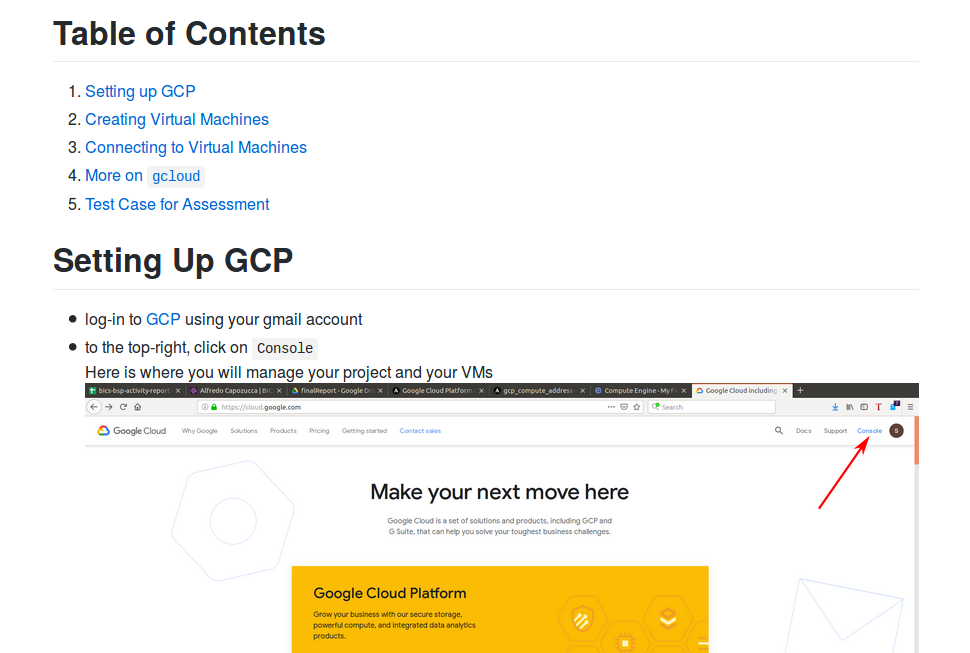
\includegraphics[width=.5\textwidth]{Images/markdown-showcase.png}
%     \caption{Markdown example}
%     \label{fig:markdown}
% \end{figure}

Here we have, for instance, the table of contents which is followed by
a few items colored in blue. This means that you can click on it to
jump some place else. For the table of content, it makes you jump to
the corresponding section in the tutorial. Also, in the first bullet
point in the figure, you can see that \textit{GCP} is colored blue.
This one will actually take you to the Google Cloud Platform.  We used
this all throughout the tutorial to send the reader, in case of need,
to a specific section to get a refresher or some additional
information.

\subsection{Assessment ($\pm$ 15\% of section's words)}
% Due to time constraints, we are not going to use the Excalibur
% Tutorial as our test case. Instead, we will do a few basic tasks to
% check if the machine is usable.

% We are going to download and install Remarkable for this purpose.
% Since downloading and installing software will be part of the tasks
% required to set up Excalibur, this seems like a good trade off.

% Further, to make this test case more adapted to a real life situation,
% we will be running one or two Youtube videos in the background as well
% as having a word editor opened while doing the installation.

% If we give our machine enough resources to work properly, then these
% tasks should be doable without any major problems.

We will evaluate the solution with regards to the non-functional
requirements to check how well these have been tackled. Admittedly,
the only part of the final solution that has not been solved yet is to
automatically ensure SSH and RDP\footnote{Remote Desktop Protocol is
used for sharing the Desktop of the instance} access once the instance
is created.  So this is a step which the DevOps engineer needs to do
manually before being able to respectively provision the machine and
set up the Excalibur Environment.

Also, we will consider that the DevOps engineer uses the solution
provided on GitHub more than once since the first time around there
are quite a few things to set up but after that, the deployment of new
instances is quite fast. So for the evaluation we will not consider
the things you have to do the very first time.

We will use the following scale ranging from handled the worst to
handled the best for evaluation purposes: \verb|--|, \verb|-|,
\verb|+|, \verb|++|.

\begin{enumerate}

	\item \textbf{Operability}.  In order to evaluate
	this we will take into consideration all the things the DevOps
	engineer must be able to do beforehand in order to tackle the
	given solution.

	For our solution, the DevOps engineer must at least know how to
	set up GCP and a project, how to set up the gcloud command line
	tool and how to get SSH access to the instances. After that, the
	scripts handle pretty much everything. Granted, the tutorial we
	provided gives step by step instructions for these tasks. Thus we
	conclude that the operability is \verb|+|.

	\item \textbf{Efficiency}. In order to evaluate
	this non-functional requirement, we will look at the amount of
	steps necessary to acquire the Virtual Machine and get them ready
	for the Excalibur Environment. We will orient ourselves on the
	tutorial that will be presented along side the script.

	If you want to create the virtual machine manually it will take
	you 3 steps. If you opt for the script or gcloud tool there is
	only 1 step. Although the gcloud tool might take you a few more
	steps to find the right things to put in the flags.

	For provisioning you have to set up SSH access manually and
	afterwards you need to set up RDP access as well. These two steps
	might be a little cumbersome. So the efficiency is \verb|+|.

	\item \textbf{Satisfaction}.  In order to evaluate
	this, we will again look at the amount of steps necessary but also
	at the time required to execute them.  This is due to the fact
	that more and lengthy steps to follow decrease the ease and speed
	at which you can repeat a given solution.

	We have two steps on SSH and RDP that need to be done manually and
	that may be a little annoying, but at the same time we give the
	user the possibility to use an Excalibur Environment with great
	ease. In fact, the Excalibur user does not have to do anything at
	all. Despite the two manual interactions we will say, thanks to
	the great satisfaction on the user's side, that satisfaction is
	\verb|++|.

	\item \textbf{Maintainability}.  For evaluation of this
	non-functional requirement, we look at how difficult and how much
	effort it may take for the DevOps engineer to tweak the creation
	and provisioning.

	The two steps that require manual intervention, namely the SSH and
	RDP setup, do not give rise to maintainability issues because you
	set them up once and there is nothing to worry about anymore.
	Added to the fact that everything is handled by scripts which you
	can go and edit, we conclude that maintainability is \verb|++|.

	\item \textbf{Reliability}.  For our evaluation purpose, we will
	try to look at how many things can go wrong during the Virtual
	Machine creation as well as setting up remote access. So the fewer
	things there are that can go wrong, the more reliable the solution
	will be.

	Except for the two steps in setting up SSH and RDP nothing can
	really go wrong because the script handles the rest and we are
	granted with a certain level of reliability, concerning the
	virtual machines, on GCP's part. For setting up SSH there are not
	too many things that can go wrong considering there are not a lot
	of steps and they are rather simple. However the RDP setup
	requires a few steps that may or may not demand a little more
	attention, since you need to have a look at one or the other
	configuration file.  Hence we will say that reliability is
	\verb|+|.

	\item \textbf{Adaptability}. To evaluate this non-functional
	requirement, we will consider the ease with which you can adapt an
	instance to a given situation.
	
	Due to the fact that instances are not physical, we can pretty
	easily tweak their properties. We should note that this is not as
	easily accomplished with physical machines as with virtual
	machines. Hence adaptability is \verb|++|.

	\item \textbf{Performance efficiency}. For evaluation purpose, we
	will look at how good of a performance we can achieve with a given
	set of resources.

	Thanks to the fact that we can tweak the instance's
	properties\footnote{We are assuming that the servers where our
	instances are running on have enough resources to allow us to do
	this}, like resources, we have the ability to try and fiddle
	around with the amount of resources until we find a specification
	that yields the greatest performance with the least amount of
	resources. Due to the potential fiddling, we will say that
	performance efficiency is \verb|+|.

\end{enumerate}

The summary table \ref{tab:NFR} gives an overview of this
non-functional requirement evaluation.

\begin{table}
\centering
\begin{tabular}{l | c}
		 Non-Functional Requirement & Evaluation \\\hline
		 Operability & \verb|+| \\
		 Efficiency & \verb|+| \\
		 Satisfaction & \verb|++| \\
		 Maintainability & \verb|++| \\
		 Reliability & \verb|+| \\
		 Adaptability & \verb|++| \\
		 Performance efficiency & \verb|+|
	\end{tabular}
	\caption{NFR summary table}
	\label{tab:NFR}
\end{table}


\section{Scientific Deliverable 2 -- Private/Public Keys for SSH
access}
% {\color{gray}
For each technical deliverable targeted in
section~\ref{subsec:deliverables} provide a full section with all the
subsections described below.  The cumulative volume of all deliverable
sections represents 75\% of the paper's volume in words. Volumes below
are indicated relative the the section.
}

\subsection{Requirements ($\pm$ 15\% of section's words)}
The main techical deliverable for this BSP, is a solution that
automates the process of creating and provisioning virtual machines on
the Google Cloud Platform in order to host an Excalibur Environment on
it. Part of this solution is based on earlier results that have been
worked out in the previous semester. 

The functional requirement of this solution is to set up a new
Excalibur Environment as fast as possible while needing the least
amount of effort. We want as much of the set up as possible to be done
by simply executing the provided scripts.

The non-functional requirements are more numerous. We want to tackle:
\begin{enumerate}

	\item \textbf{Operability}, which determines how accessible and
		easy to use the solution is.

	\item \textbf{Efficiency}, which considers the amount of effort
		necessary to bring the solution to use.
		
	\item \textbf{Satisfaction}, informs us on the degree to which user needs
		are satisfied when a product or system is used in a specified
		context of use.
		
	
	\item \textbf{Maintainability}, considers the ease at which the developer
		can change aspects of the Virtual Machine creation and the provisioning.
		
	\item \textbf{Reliability}, tells us whether or not our solution
		is reliable. In other words: Does it give the same result in
		successive trials?
		
\end{enumerate}

This technical deliverable is targeted towards a DevOps engineer, who
is in charge of setting up these machines. The Excalibur user should
not have to deal with anything regarding the production of the final
product, namely the Excalibur Environment.

\subsection{Design ($\pm$ 30\% of section's words)}
In order to learn about GCP and understand how it works, we decided to
look for online courses and tutorials. These courses were meant to
teach us the basic usage of the platform as well as a few basic
concepts related to it. 

The first
tutorial\footnote{\url{https://bics.udemy.com/introduction-to-cloud-computing/learn/v4/overview}}
we watched was a single long video that briefly explained all the
concepts related to GCP, thus giving a first overview of what we will
be dealing with.

After that, we watched two tutorial series, although not in their
entirety, created by Google
themselves\footnote{\url{https://www.coursera.org/learn/gcp-fundamentals/home/welcome}
and
\url{https://www.coursera.org/learn/gcp-infrastructure-foundation/home/welcome}}
that gave a more detailed insight into the various concepts and how
they work in practice through a set of exercises.

Finally, when first accessing GCP a message popped up proposing a
guided tour through the platform. This was basically an interactive
tutorial that showed us how to navigate the platform and where to find
the most important tools.

\subsection{Production ($\pm$ 40\% of section's words)}
% {\color{gray}
% Provide descriptions of the deliverables concrete production. It must
% present part of the deliverable (e.g. source code extracts, scientific
% work extracts, \ldots) to illustrate and explain its actual
% production.
% }

The tutorial has been written in Markdown. I decided to go with
Markdown because it is quite easy to use and you can add it to a
GitHub repository.  Considering that we will put this solution onto
GitHub\footnote{See appendix section \ref{app:github}}, this seemed
like a very good idea. This way the tutorial is included with the
solution and is presented nicely. Find more technical information in
the appendix section \ref{app:markdown}.

To begin with, we needed a way to write Markdown files. I used to
write my Markdown files with
ReText\footnote{\url{https://github.com/retext-project/retext}}
however I had a few issues with it and the output did not look all
that nice. I tried switching to Vim, which has a pluggin for
supporting real-time Markdown rendering in a
browser\footnote{\url{https://github.com/suan/vim-instant-markdown}}
but again I had an issue here and it did not even seem to work. I kept
searching a bit more and I found
Remarkable\footnote{\url{https://remarkableapp.github.io/}} which was
pretty good for the purposes of writing the tutorial.

Once we were set for writing the tutorial, we began with writing down
things we already knew how to do. So we build the tutorial as we went,
feeding it with new information as we learnt and discovered it.

Some parts of the tutorial required us to completely restart from
scratch because once you have everything set up, there are things that
differ compared to doing it the first time around. Especially all the
things related to GCP have been done from scratch to show to the user
everything he needs to know to get started. Once everything is set up
there are fewer things to worry about, but they are important to
highlight the first time around.

Markdown has the ability to insert images, so we used it to our
advantage to illustrate a lot of things. See an example of a picture
in figure \ref{fig:markdown}. Furthermore, it allows us to include
references, either external or internal ones. So we can have
references to other websites or to other sections within the file.

We also used this to our advantage, to introduce various other
notions, without interrupting the flow of the text. See figure
\ref{fig:markdown}.

% \begin{figure}
%     \centering
%     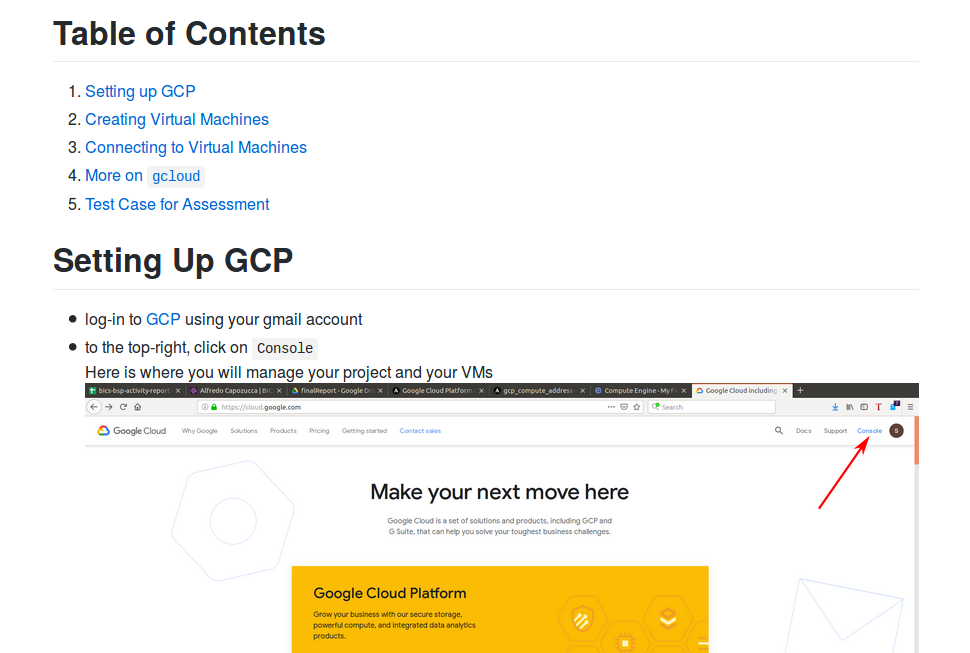
\includegraphics[width=.5\textwidth]{Images/markdown-showcase.png}
%     \caption{Markdown example}
%     \label{fig:markdown}
% \end{figure}

Here we have, for instance, the table of contents which is followed by
a few items colored in blue. This means that you can click on it to
jump some place else. For the table of content, it makes you jump to
the corresponding section in the tutorial. Also, in the first bullet
point in the figure, you can see that \textit{GCP} is colored blue.
This one will actually take you to the Google Cloud Platform.  We used
this all throughout the tutorial to send the reader, in case of need,
to a specific section to get a refresher or some additional
information.

\subsection{Assessment ($\pm$ 15\% of section's words)}
% Due to time constraints, we are not going to use the Excalibur
% Tutorial as our test case. Instead, we will do a few basic tasks to
% check if the machine is usable.

% We are going to download and install Remarkable for this purpose.
% Since downloading and installing software will be part of the tasks
% required to set up Excalibur, this seems like a good trade off.

% Further, to make this test case more adapted to a real life situation,
% we will be running one or two Youtube videos in the background as well
% as having a word editor opened while doing the installation.

% If we give our machine enough resources to work properly, then these
% tasks should be doable without any major problems.

We will evaluate the solution with regards to the non-functional
requirements to check how well these have been tackled. Admittedly,
the only part of the final solution that has not been solved yet is to
automatically ensure SSH and RDP\footnote{Remote Desktop Protocol is
used for sharing the Desktop of the instance} access once the instance
is created.  So this is a step which the DevOps engineer needs to do
manually before being able to respectively provision the machine and
set up the Excalibur Environment.

Also, we will consider that the DevOps engineer uses the solution
provided on GitHub more than once since the first time around there
are quite a few things to set up but after that, the deployment of new
instances is quite fast. So for the evaluation we will not consider
the things you have to do the very first time.

We will use the following scale ranging from handled the worst to
handled the best for evaluation purposes: \verb|--|, \verb|-|,
\verb|+|, \verb|++|.

\begin{enumerate}

	\item \textbf{Operability}.  In order to evaluate
	this we will take into consideration all the things the DevOps
	engineer must be able to do beforehand in order to tackle the
	given solution.

	For our solution, the DevOps engineer must at least know how to
	set up GCP and a project, how to set up the gcloud command line
	tool and how to get SSH access to the instances. After that, the
	scripts handle pretty much everything. Granted, the tutorial we
	provided gives step by step instructions for these tasks. Thus we
	conclude that the operability is \verb|+|.

	\item \textbf{Efficiency}. In order to evaluate
	this non-functional requirement, we will look at the amount of
	steps necessary to acquire the Virtual Machine and get them ready
	for the Excalibur Environment. We will orient ourselves on the
	tutorial that will be presented along side the script.

	If you want to create the virtual machine manually it will take
	you 3 steps. If you opt for the script or gcloud tool there is
	only 1 step. Although the gcloud tool might take you a few more
	steps to find the right things to put in the flags.

	For provisioning you have to set up SSH access manually and
	afterwards you need to set up RDP access as well. These two steps
	might be a little cumbersome. So the efficiency is \verb|+|.

	\item \textbf{Satisfaction}.  In order to evaluate
	this, we will again look at the amount of steps necessary but also
	at the time required to execute them.  This is due to the fact
	that more and lengthy steps to follow decrease the ease and speed
	at which you can repeat a given solution.

	We have two steps on SSH and RDP that need to be done manually and
	that may be a little annoying, but at the same time we give the
	user the possibility to use an Excalibur Environment with great
	ease. In fact, the Excalibur user does not have to do anything at
	all. Despite the two manual interactions we will say, thanks to
	the great satisfaction on the user's side, that satisfaction is
	\verb|++|.

	\item \textbf{Maintainability}.  For evaluation of this
	non-functional requirement, we look at how difficult and how much
	effort it may take for the DevOps engineer to tweak the creation
	and provisioning.

	The two steps that require manual intervention, namely the SSH and
	RDP setup, do not give rise to maintainability issues because you
	set them up once and there is nothing to worry about anymore.
	Added to the fact that everything is handled by scripts which you
	can go and edit, we conclude that maintainability is \verb|++|.

	\item \textbf{Reliability}.  For our evaluation purpose, we will
	try to look at how many things can go wrong during the Virtual
	Machine creation as well as setting up remote access. So the fewer
	things there are that can go wrong, the more reliable the solution
	will be.

	Except for the two steps in setting up SSH and RDP nothing can
	really go wrong because the script handles the rest and we are
	granted with a certain level of reliability, concerning the
	virtual machines, on GCP's part. For setting up SSH there are not
	too many things that can go wrong considering there are not a lot
	of steps and they are rather simple. However the RDP setup
	requires a few steps that may or may not demand a little more
	attention, since you need to have a look at one or the other
	configuration file.  Hence we will say that reliability is
	\verb|+|.

	\item \textbf{Adaptability}. To evaluate this non-functional
	requirement, we will consider the ease with which you can adapt an
	instance to a given situation.
	
	Due to the fact that instances are not physical, we can pretty
	easily tweak their properties. We should note that this is not as
	easily accomplished with physical machines as with virtual
	machines. Hence adaptability is \verb|++|.

	\item \textbf{Performance efficiency}. For evaluation purpose, we
	will look at how good of a performance we can achieve with a given
	set of resources.

	Thanks to the fact that we can tweak the instance's
	properties\footnote{We are assuming that the servers where our
	instances are running on have enough resources to allow us to do
	this}, like resources, we have the ability to try and fiddle
	around with the amount of resources until we find a specification
	that yields the greatest performance with the least amount of
	resources. Due to the potential fiddling, we will say that
	performance efficiency is \verb|+|.

\end{enumerate}

The summary table \ref{tab:NFR} gives an overview of this
non-functional requirement evaluation.

\begin{table}
\centering
\begin{tabular}{l | c}
		 Non-Functional Requirement & Evaluation \\\hline
		 Operability & \verb|+| \\
		 Efficiency & \verb|+| \\
		 Satisfaction & \verb|++| \\
		 Maintainability & \verb|++| \\
		 Reliability & \verb|+| \\
		 Adaptability & \verb|++| \\
		 Performance efficiency & \verb|+|
	\end{tabular}
	\caption{NFR summary table}
	\label{tab:NFR}
\end{table}


\section{Scientific Deliverable 3 -- Tutorial}
% {\color{gray}
For each technical deliverable targeted in
section~\ref{subsec:deliverables} provide a full section with all the
subsections described below.  The cumulative volume of all deliverable
sections represents 75\% of the paper's volume in words. Volumes below
are indicated relative the the section.
}

\subsection{Requirements ($\pm$ 15\% of section's words)}
The main techical deliverable for this BSP, is a solution that
automates the process of creating and provisioning virtual machines on
the Google Cloud Platform in order to host an Excalibur Environment on
it. Part of this solution is based on earlier results that have been
worked out in the previous semester. 

The functional requirement of this solution is to set up a new
Excalibur Environment as fast as possible while needing the least
amount of effort. We want as much of the set up as possible to be done
by simply executing the provided scripts.

The non-functional requirements are more numerous. We want to tackle:
\begin{enumerate}

	\item \textbf{Operability}, which determines how accessible and
		easy to use the solution is.

	\item \textbf{Efficiency}, which considers the amount of effort
		necessary to bring the solution to use.
		
	\item \textbf{Satisfaction}, informs us on the degree to which user needs
		are satisfied when a product or system is used in a specified
		context of use.
		
	
	\item \textbf{Maintainability}, considers the ease at which the developer
		can change aspects of the Virtual Machine creation and the provisioning.
		
	\item \textbf{Reliability}, tells us whether or not our solution
		is reliable. In other words: Does it give the same result in
		successive trials?
		
\end{enumerate}

This technical deliverable is targeted towards a DevOps engineer, who
is in charge of setting up these machines. The Excalibur user should
not have to deal with anything regarding the production of the final
product, namely the Excalibur Environment.

\subsection{Design ($\pm$ 30\% of section's words)}
In order to learn about GCP and understand how it works, we decided to
look for online courses and tutorials. These courses were meant to
teach us the basic usage of the platform as well as a few basic
concepts related to it. 

The first
tutorial\footnote{\url{https://bics.udemy.com/introduction-to-cloud-computing/learn/v4/overview}}
we watched was a single long video that briefly explained all the
concepts related to GCP, thus giving a first overview of what we will
be dealing with.

After that, we watched two tutorial series, although not in their
entirety, created by Google
themselves\footnote{\url{https://www.coursera.org/learn/gcp-fundamentals/home/welcome}
and
\url{https://www.coursera.org/learn/gcp-infrastructure-foundation/home/welcome}}
that gave a more detailed insight into the various concepts and how
they work in practice through a set of exercises.

Finally, when first accessing GCP a message popped up proposing a
guided tour through the platform. This was basically an interactive
tutorial that showed us how to navigate the platform and where to find
the most important tools.

\subsection{Production ($\pm$ 40\% of section's words)}
% {\color{gray}
% Provide descriptions of the deliverables concrete production. It must
% present part of the deliverable (e.g. source code extracts, scientific
% work extracts, \ldots) to illustrate and explain its actual
% production.
% }

The tutorial has been written in Markdown. I decided to go with
Markdown because it is quite easy to use and you can add it to a
GitHub repository.  Considering that we will put this solution onto
GitHub\footnote{See appendix section \ref{app:github}}, this seemed
like a very good idea. This way the tutorial is included with the
solution and is presented nicely. Find more technical information in
the appendix section \ref{app:markdown}.

To begin with, we needed a way to write Markdown files. I used to
write my Markdown files with
ReText\footnote{\url{https://github.com/retext-project/retext}}
however I had a few issues with it and the output did not look all
that nice. I tried switching to Vim, which has a pluggin for
supporting real-time Markdown rendering in a
browser\footnote{\url{https://github.com/suan/vim-instant-markdown}}
but again I had an issue here and it did not even seem to work. I kept
searching a bit more and I found
Remarkable\footnote{\url{https://remarkableapp.github.io/}} which was
pretty good for the purposes of writing the tutorial.

Once we were set for writing the tutorial, we began with writing down
things we already knew how to do. So we build the tutorial as we went,
feeding it with new information as we learnt and discovered it.

Some parts of the tutorial required us to completely restart from
scratch because once you have everything set up, there are things that
differ compared to doing it the first time around. Especially all the
things related to GCP have been done from scratch to show to the user
everything he needs to know to get started. Once everything is set up
there are fewer things to worry about, but they are important to
highlight the first time around.

Markdown has the ability to insert images, so we used it to our
advantage to illustrate a lot of things. See an example of a picture
in figure \ref{fig:markdown}. Furthermore, it allows us to include
references, either external or internal ones. So we can have
references to other websites or to other sections within the file.

We also used this to our advantage, to introduce various other
notions, without interrupting the flow of the text. See figure
\ref{fig:markdown}.

% \begin{figure}
%     \centering
%     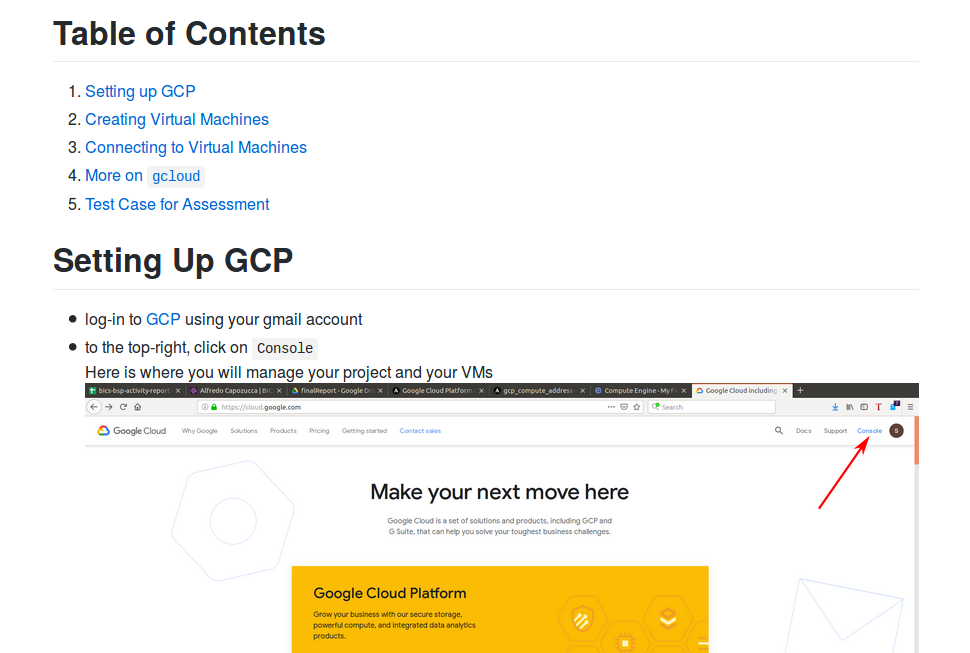
\includegraphics[width=.5\textwidth]{Images/markdown-showcase.png}
%     \caption{Markdown example}
%     \label{fig:markdown}
% \end{figure}

Here we have, for instance, the table of contents which is followed by
a few items colored in blue. This means that you can click on it to
jump some place else. For the table of content, it makes you jump to
the corresponding section in the tutorial. Also, in the first bullet
point in the figure, you can see that \textit{GCP} is colored blue.
This one will actually take you to the Google Cloud Platform.  We used
this all throughout the tutorial to send the reader, in case of need,
to a specific section to get a refresher or some additional
information.

\subsection{Assessment ($\pm$ 15\% of section's words)}
% Due to time constraints, we are not going to use the Excalibur
% Tutorial as our test case. Instead, we will do a few basic tasks to
% check if the machine is usable.

% We are going to download and install Remarkable for this purpose.
% Since downloading and installing software will be part of the tasks
% required to set up Excalibur, this seems like a good trade off.

% Further, to make this test case more adapted to a real life situation,
% we will be running one or two Youtube videos in the background as well
% as having a word editor opened while doing the installation.

% If we give our machine enough resources to work properly, then these
% tasks should be doable without any major problems.

We will evaluate the solution with regards to the non-functional
requirements to check how well these have been tackled. Admittedly,
the only part of the final solution that has not been solved yet is to
automatically ensure SSH and RDP\footnote{Remote Desktop Protocol is
used for sharing the Desktop of the instance} access once the instance
is created.  So this is a step which the DevOps engineer needs to do
manually before being able to respectively provision the machine and
set up the Excalibur Environment.

Also, we will consider that the DevOps engineer uses the solution
provided on GitHub more than once since the first time around there
are quite a few things to set up but after that, the deployment of new
instances is quite fast. So for the evaluation we will not consider
the things you have to do the very first time.

We will use the following scale ranging from handled the worst to
handled the best for evaluation purposes: \verb|--|, \verb|-|,
\verb|+|, \verb|++|.

\begin{enumerate}

	\item \textbf{Operability}.  In order to evaluate
	this we will take into consideration all the things the DevOps
	engineer must be able to do beforehand in order to tackle the
	given solution.

	For our solution, the DevOps engineer must at least know how to
	set up GCP and a project, how to set up the gcloud command line
	tool and how to get SSH access to the instances. After that, the
	scripts handle pretty much everything. Granted, the tutorial we
	provided gives step by step instructions for these tasks. Thus we
	conclude that the operability is \verb|+|.

	\item \textbf{Efficiency}. In order to evaluate
	this non-functional requirement, we will look at the amount of
	steps necessary to acquire the Virtual Machine and get them ready
	for the Excalibur Environment. We will orient ourselves on the
	tutorial that will be presented along side the script.

	If you want to create the virtual machine manually it will take
	you 3 steps. If you opt for the script or gcloud tool there is
	only 1 step. Although the gcloud tool might take you a few more
	steps to find the right things to put in the flags.

	For provisioning you have to set up SSH access manually and
	afterwards you need to set up RDP access as well. These two steps
	might be a little cumbersome. So the efficiency is \verb|+|.

	\item \textbf{Satisfaction}.  In order to evaluate
	this, we will again look at the amount of steps necessary but also
	at the time required to execute them.  This is due to the fact
	that more and lengthy steps to follow decrease the ease and speed
	at which you can repeat a given solution.

	We have two steps on SSH and RDP that need to be done manually and
	that may be a little annoying, but at the same time we give the
	user the possibility to use an Excalibur Environment with great
	ease. In fact, the Excalibur user does not have to do anything at
	all. Despite the two manual interactions we will say, thanks to
	the great satisfaction on the user's side, that satisfaction is
	\verb|++|.

	\item \textbf{Maintainability}.  For evaluation of this
	non-functional requirement, we look at how difficult and how much
	effort it may take for the DevOps engineer to tweak the creation
	and provisioning.

	The two steps that require manual intervention, namely the SSH and
	RDP setup, do not give rise to maintainability issues because you
	set them up once and there is nothing to worry about anymore.
	Added to the fact that everything is handled by scripts which you
	can go and edit, we conclude that maintainability is \verb|++|.

	\item \textbf{Reliability}.  For our evaluation purpose, we will
	try to look at how many things can go wrong during the Virtual
	Machine creation as well as setting up remote access. So the fewer
	things there are that can go wrong, the more reliable the solution
	will be.

	Except for the two steps in setting up SSH and RDP nothing can
	really go wrong because the script handles the rest and we are
	granted with a certain level of reliability, concerning the
	virtual machines, on GCP's part. For setting up SSH there are not
	too many things that can go wrong considering there are not a lot
	of steps and they are rather simple. However the RDP setup
	requires a few steps that may or may not demand a little more
	attention, since you need to have a look at one or the other
	configuration file.  Hence we will say that reliability is
	\verb|+|.

	\item \textbf{Adaptability}. To evaluate this non-functional
	requirement, we will consider the ease with which you can adapt an
	instance to a given situation.
	
	Due to the fact that instances are not physical, we can pretty
	easily tweak their properties. We should note that this is not as
	easily accomplished with physical machines as with virtual
	machines. Hence adaptability is \verb|++|.

	\item \textbf{Performance efficiency}. For evaluation purpose, we
	will look at how good of a performance we can achieve with a given
	set of resources.

	Thanks to the fact that we can tweak the instance's
	properties\footnote{We are assuming that the servers where our
	instances are running on have enough resources to allow us to do
	this}, like resources, we have the ability to try and fiddle
	around with the amount of resources until we find a specification
	that yields the greatest performance with the least amount of
	resources. Due to the potential fiddling, we will say that
	performance efficiency is \verb|+|.

\end{enumerate}

The summary table \ref{tab:NFR} gives an overview of this
non-functional requirement evaluation.

\begin{table}
\centering
\begin{tabular}{l | c}
		 Non-Functional Requirement & Evaluation \\\hline
		 Operability & \verb|+| \\
		 Efficiency & \verb|+| \\
		 Satisfaction & \verb|++| \\
		 Maintainability & \verb|++| \\
		 Reliability & \verb|+| \\
		 Adaptability & \verb|++| \\
		 Performance efficiency & \verb|+|
	\end{tabular}
	\caption{NFR summary table}
	\label{tab:NFR}
\end{table}


% \section{A Scientific Deliverable 1}
% {\color{gray}
For each technical deliverable targeted in
section~\ref{subsec:deliverables} provide a full section with all the
subsections described below.  The cumulative volume of all deliverable
sections represents 75\% of the paper's volume in words. Volumes below
are indicated relative the the section.
}

% \subsection{Requirements ($\pm$ 15\% of section's words)}
% The main techical deliverable for this BSP, is a solution that
automates the process of creating and provisioning virtual machines on
the Google Cloud Platform in order to host an Excalibur Environment on
it. Part of this solution is based on earlier results that have been
worked out in the previous semester. 

The functional requirement of this solution is to set up a new
Excalibur Environment as fast as possible while needing the least
amount of effort. We want as much of the set up as possible to be done
by simply executing the provided scripts.

The non-functional requirements are more numerous. We want to tackle:
\begin{enumerate}

	\item \textbf{Operability}, which determines how accessible and
		easy to use the solution is.

	\item \textbf{Efficiency}, which considers the amount of effort
		necessary to bring the solution to use.
		
	\item \textbf{Satisfaction}, informs us on the degree to which user needs
		are satisfied when a product or system is used in a specified
		context of use.
		
	
	\item \textbf{Maintainability}, considers the ease at which the developer
		can change aspects of the Virtual Machine creation and the provisioning.
		
	\item \textbf{Reliability}, tells us whether or not our solution
		is reliable. In other words: Does it give the same result in
		successive trials?
		
\end{enumerate}

This technical deliverable is targeted towards a DevOps engineer, who
is in charge of setting up these machines. The Excalibur user should
not have to deal with anything regarding the production of the final
product, namely the Excalibur Environment.

% \subsection{Design ($\pm$ 30\% of section's words)}
% In order to learn about GCP and understand how it works, we decided to
look for online courses and tutorials. These courses were meant to
teach us the basic usage of the platform as well as a few basic
concepts related to it. 

The first
tutorial\footnote{\url{https://bics.udemy.com/introduction-to-cloud-computing/learn/v4/overview}}
we watched was a single long video that briefly explained all the
concepts related to GCP, thus giving a first overview of what we will
be dealing with.

After that, we watched two tutorial series, although not in their
entirety, created by Google
themselves\footnote{\url{https://www.coursera.org/learn/gcp-fundamentals/home/welcome}
and
\url{https://www.coursera.org/learn/gcp-infrastructure-foundation/home/welcome}}
that gave a more detailed insight into the various concepts and how
they work in practice through a set of exercises.

Finally, when first accessing GCP a message popped up proposing a
guided tour through the platform. This was basically an interactive
tutorial that showed us how to navigate the platform and where to find
the most important tools.

% \subsection{Production ($\pm$ 40\% of section's words)}
% % {\color{gray}
% Provide descriptions of the deliverables concrete production. It must
% present part of the deliverable (e.g. source code extracts, scientific
% work extracts, \ldots) to illustrate and explain its actual
% production.
% }

The tutorial has been written in Markdown. I decided to go with
Markdown because it is quite easy to use and you can add it to a
GitHub repository.  Considering that we will put this solution onto
GitHub\footnote{See appendix section \ref{app:github}}, this seemed
like a very good idea. This way the tutorial is included with the
solution and is presented nicely. Find more technical information in
the appendix section \ref{app:markdown}.

To begin with, we needed a way to write Markdown files. I used to
write my Markdown files with
ReText\footnote{\url{https://github.com/retext-project/retext}}
however I had a few issues with it and the output did not look all
that nice. I tried switching to Vim, which has a pluggin for
supporting real-time Markdown rendering in a
browser\footnote{\url{https://github.com/suan/vim-instant-markdown}}
but again I had an issue here and it did not even seem to work. I kept
searching a bit more and I found
Remarkable\footnote{\url{https://remarkableapp.github.io/}} which was
pretty good for the purposes of writing the tutorial.

Once we were set for writing the tutorial, we began with writing down
things we already knew how to do. So we build the tutorial as we went,
feeding it with new information as we learnt and discovered it.

Some parts of the tutorial required us to completely restart from
scratch because once you have everything set up, there are things that
differ compared to doing it the first time around. Especially all the
things related to GCP have been done from scratch to show to the user
everything he needs to know to get started. Once everything is set up
there are fewer things to worry about, but they are important to
highlight the first time around.

Markdown has the ability to insert images, so we used it to our
advantage to illustrate a lot of things. See an example of a picture
in figure \ref{fig:markdown}. Furthermore, it allows us to include
references, either external or internal ones. So we can have
references to other websites or to other sections within the file.

We also used this to our advantage, to introduce various other
notions, without interrupting the flow of the text. See figure
\ref{fig:markdown}.

% \begin{figure}
%     \centering
%     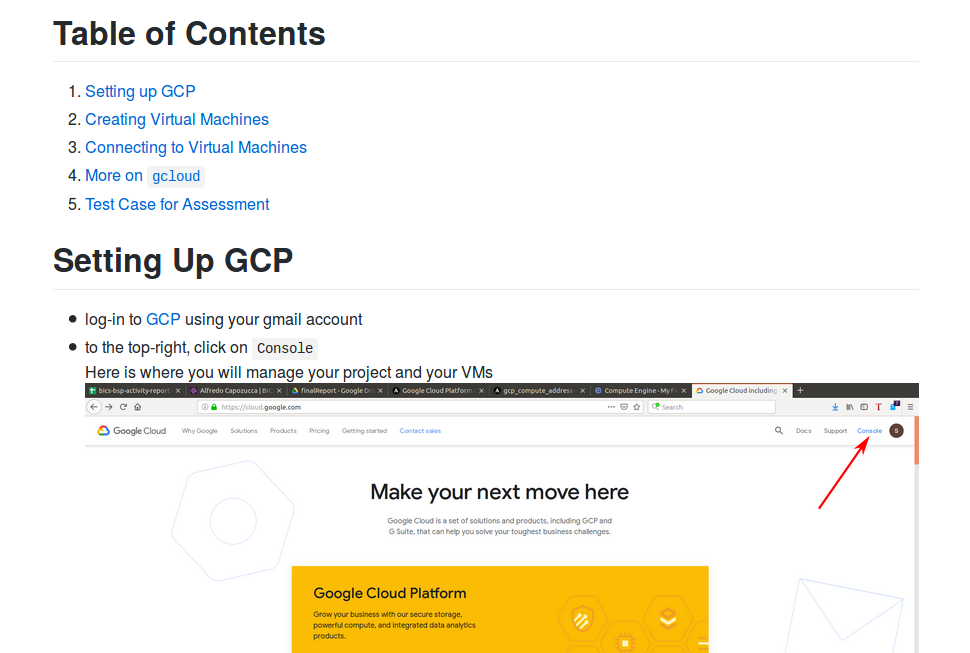
\includegraphics[width=.5\textwidth]{Images/markdown-showcase.png}
%     \caption{Markdown example}
%     \label{fig:markdown}
% \end{figure}

Here we have, for instance, the table of contents which is followed by
a few items colored in blue. This means that you can click on it to
jump some place else. For the table of content, it makes you jump to
the corresponding section in the tutorial. Also, in the first bullet
point in the figure, you can see that \textit{GCP} is colored blue.
This one will actually take you to the Google Cloud Platform.  We used
this all throughout the tutorial to send the reader, in case of need,
to a specific section to get a refresher or some additional
information.

% \subsection{Assessment ($\pm$ 15\% of section's words)}
% % Due to time constraints, we are not going to use the Excalibur
% Tutorial as our test case. Instead, we will do a few basic tasks to
% check if the machine is usable.

% We are going to download and install Remarkable for this purpose.
% Since downloading and installing software will be part of the tasks
% required to set up Excalibur, this seems like a good trade off.

% Further, to make this test case more adapted to a real life situation,
% we will be running one or two Youtube videos in the background as well
% as having a word editor opened while doing the installation.

% If we give our machine enough resources to work properly, then these
% tasks should be doable without any major problems.

We will evaluate the solution with regards to the non-functional
requirements to check how well these have been tackled. Admittedly,
the only part of the final solution that has not been solved yet is to
automatically ensure SSH and RDP\footnote{Remote Desktop Protocol is
used for sharing the Desktop of the instance} access once the instance
is created.  So this is a step which the DevOps engineer needs to do
manually before being able to respectively provision the machine and
set up the Excalibur Environment.

Also, we will consider that the DevOps engineer uses the solution
provided on GitHub more than once since the first time around there
are quite a few things to set up but after that, the deployment of new
instances is quite fast. So for the evaluation we will not consider
the things you have to do the very first time.

We will use the following scale ranging from handled the worst to
handled the best for evaluation purposes: \verb|--|, \verb|-|,
\verb|+|, \verb|++|.

\begin{enumerate}

	\item \textbf{Operability}.  In order to evaluate
	this we will take into consideration all the things the DevOps
	engineer must be able to do beforehand in order to tackle the
	given solution.

	For our solution, the DevOps engineer must at least know how to
	set up GCP and a project, how to set up the gcloud command line
	tool and how to get SSH access to the instances. After that, the
	scripts handle pretty much everything. Granted, the tutorial we
	provided gives step by step instructions for these tasks. Thus we
	conclude that the operability is \verb|+|.

	\item \textbf{Efficiency}. In order to evaluate
	this non-functional requirement, we will look at the amount of
	steps necessary to acquire the Virtual Machine and get them ready
	for the Excalibur Environment. We will orient ourselves on the
	tutorial that will be presented along side the script.

	If you want to create the virtual machine manually it will take
	you 3 steps. If you opt for the script or gcloud tool there is
	only 1 step. Although the gcloud tool might take you a few more
	steps to find the right things to put in the flags.

	For provisioning you have to set up SSH access manually and
	afterwards you need to set up RDP access as well. These two steps
	might be a little cumbersome. So the efficiency is \verb|+|.

	\item \textbf{Satisfaction}.  In order to evaluate
	this, we will again look at the amount of steps necessary but also
	at the time required to execute them.  This is due to the fact
	that more and lengthy steps to follow decrease the ease and speed
	at which you can repeat a given solution.

	We have two steps on SSH and RDP that need to be done manually and
	that may be a little annoying, but at the same time we give the
	user the possibility to use an Excalibur Environment with great
	ease. In fact, the Excalibur user does not have to do anything at
	all. Despite the two manual interactions we will say, thanks to
	the great satisfaction on the user's side, that satisfaction is
	\verb|++|.

	\item \textbf{Maintainability}.  For evaluation of this
	non-functional requirement, we look at how difficult and how much
	effort it may take for the DevOps engineer to tweak the creation
	and provisioning.

	The two steps that require manual intervention, namely the SSH and
	RDP setup, do not give rise to maintainability issues because you
	set them up once and there is nothing to worry about anymore.
	Added to the fact that everything is handled by scripts which you
	can go and edit, we conclude that maintainability is \verb|++|.

	\item \textbf{Reliability}.  For our evaluation purpose, we will
	try to look at how many things can go wrong during the Virtual
	Machine creation as well as setting up remote access. So the fewer
	things there are that can go wrong, the more reliable the solution
	will be.

	Except for the two steps in setting up SSH and RDP nothing can
	really go wrong because the script handles the rest and we are
	granted with a certain level of reliability, concerning the
	virtual machines, on GCP's part. For setting up SSH there are not
	too many things that can go wrong considering there are not a lot
	of steps and they are rather simple. However the RDP setup
	requires a few steps that may or may not demand a little more
	attention, since you need to have a look at one or the other
	configuration file.  Hence we will say that reliability is
	\verb|+|.

	\item \textbf{Adaptability}. To evaluate this non-functional
	requirement, we will consider the ease with which you can adapt an
	instance to a given situation.
	
	Due to the fact that instances are not physical, we can pretty
	easily tweak their properties. We should note that this is not as
	easily accomplished with physical machines as with virtual
	machines. Hence adaptability is \verb|++|.

	\item \textbf{Performance efficiency}. For evaluation purpose, we
	will look at how good of a performance we can achieve with a given
	set of resources.

	Thanks to the fact that we can tweak the instance's
	properties\footnote{We are assuming that the servers where our
	instances are running on have enough resources to allow us to do
	this}, like resources, we have the ability to try and fiddle
	around with the amount of resources until we find a specification
	that yields the greatest performance with the least amount of
	resources. Due to the potential fiddling, we will say that
	performance efficiency is \verb|+|.

\end{enumerate}

The summary table \ref{tab:NFR} gives an overview of this
non-functional requirement evaluation.

\begin{table}
\centering
\begin{tabular}{l | c}
		 Non-Functional Requirement & Evaluation \\\hline
		 Operability & \verb|+| \\
		 Efficiency & \verb|+| \\
		 Satisfaction & \verb|++| \\
		 Maintainability & \verb|++| \\
		 Reliability & \verb|+| \\
		 Adaptability & \verb|++| \\
		 Performance efficiency & \verb|+|
	\end{tabular}
	\caption{NFR summary table}
	\label{tab:NFR}
\end{table}


\section{Technical Deliverable -- Provisioning}
% {\color{gray}
For each technical deliverable targeted in
section~\ref{subsec:deliverables} provide a full section with all the
subsections described below.  The cumulative volume of all deliverable
sections represents 75\% of the paper's volume in words. Volumes below
are indicated relative the the section.
}

\subsection{Requirements}% ($\pm$ 15\% of section's words)}
The main techical deliverable for this BSP, is a solution that
automates the process of creating and provisioning virtual machines on
the Google Cloud Platform in order to host an Excalibur Environment on
it. Part of this solution is based on earlier results that have been
worked out in the previous semester. 

The functional requirement of this solution is to set up a new
Excalibur Environment as fast as possible while needing the least
amount of effort. We want as much of the set up as possible to be done
by simply executing the provided scripts.

The non-functional requirements are more numerous. We want to tackle:
\begin{enumerate}

	\item \textbf{Operability}, which determines how accessible and
		easy to use the solution is.

	\item \textbf{Efficiency}, which considers the amount of effort
		necessary to bring the solution to use.
		
	\item \textbf{Satisfaction}, informs us on the degree to which user needs
		are satisfied when a product or system is used in a specified
		context of use.
		
	
	\item \textbf{Maintainability}, considers the ease at which the developer
		can change aspects of the Virtual Machine creation and the provisioning.
		
	\item \textbf{Reliability}, tells us whether or not our solution
		is reliable. In other words: Does it give the same result in
		successive trials?
		
\end{enumerate}

This technical deliverable is targeted towards a DevOps engineer, who
is in charge of setting up these machines. The Excalibur user should
not have to deal with anything regarding the production of the final
product, namely the Excalibur Environment.

\subsection{Design}% ($\pm$ 30\% of section's words)}
In order to learn about GCP and understand how it works, we decided to
look for online courses and tutorials. These courses were meant to
teach us the basic usage of the platform as well as a few basic
concepts related to it. 

The first
tutorial\footnote{\url{https://bics.udemy.com/introduction-to-cloud-computing/learn/v4/overview}}
we watched was a single long video that briefly explained all the
concepts related to GCP, thus giving a first overview of what we will
be dealing with.

After that, we watched two tutorial series, although not in their
entirety, created by Google
themselves\footnote{\url{https://www.coursera.org/learn/gcp-fundamentals/home/welcome}
and
\url{https://www.coursera.org/learn/gcp-infrastructure-foundation/home/welcome}}
that gave a more detailed insight into the various concepts and how
they work in practice through a set of exercises.

Finally, when first accessing GCP a message popped up proposing a
guided tour through the platform. This was basically an interactive
tutorial that showed us how to navigate the platform and where to find
the most important tools.

\subsection{Production}% ($\pm$ 40\% of section's words)}
% {\color{gray}
% Provide descriptions of the deliverables concrete production. It must
% present part of the deliverable (e.g. source code extracts, scientific
% work extracts, \ldots) to illustrate and explain its actual
% production.
% }

The tutorial has been written in Markdown. I decided to go with
Markdown because it is quite easy to use and you can add it to a
GitHub repository.  Considering that we will put this solution onto
GitHub\footnote{See appendix section \ref{app:github}}, this seemed
like a very good idea. This way the tutorial is included with the
solution and is presented nicely. Find more technical information in
the appendix section \ref{app:markdown}.

To begin with, we needed a way to write Markdown files. I used to
write my Markdown files with
ReText\footnote{\url{https://github.com/retext-project/retext}}
however I had a few issues with it and the output did not look all
that nice. I tried switching to Vim, which has a pluggin for
supporting real-time Markdown rendering in a
browser\footnote{\url{https://github.com/suan/vim-instant-markdown}}
but again I had an issue here and it did not even seem to work. I kept
searching a bit more and I found
Remarkable\footnote{\url{https://remarkableapp.github.io/}} which was
pretty good for the purposes of writing the tutorial.

Once we were set for writing the tutorial, we began with writing down
things we already knew how to do. So we build the tutorial as we went,
feeding it with new information as we learnt and discovered it.

Some parts of the tutorial required us to completely restart from
scratch because once you have everything set up, there are things that
differ compared to doing it the first time around. Especially all the
things related to GCP have been done from scratch to show to the user
everything he needs to know to get started. Once everything is set up
there are fewer things to worry about, but they are important to
highlight the first time around.

Markdown has the ability to insert images, so we used it to our
advantage to illustrate a lot of things. See an example of a picture
in figure \ref{fig:markdown}. Furthermore, it allows us to include
references, either external or internal ones. So we can have
references to other websites or to other sections within the file.

We also used this to our advantage, to introduce various other
notions, without interrupting the flow of the text. See figure
\ref{fig:markdown}.

% \begin{figure}
%     \centering
%     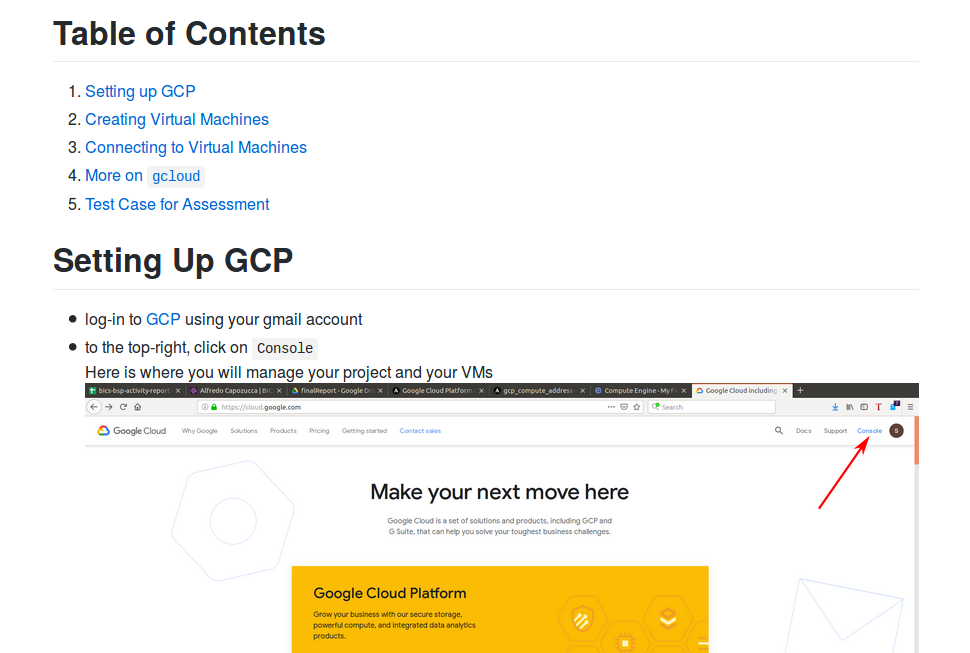
\includegraphics[width=.5\textwidth]{Images/markdown-showcase.png}
%     \caption{Markdown example}
%     \label{fig:markdown}
% \end{figure}

Here we have, for instance, the table of contents which is followed by
a few items colored in blue. This means that you can click on it to
jump some place else. For the table of content, it makes you jump to
the corresponding section in the tutorial. Also, in the first bullet
point in the figure, you can see that \textit{GCP} is colored blue.
This one will actually take you to the Google Cloud Platform.  We used
this all throughout the tutorial to send the reader, in case of need,
to a specific section to get a refresher or some additional
information.

\subsection{Assessment}% ($\pm$ 15\% of section's words)}
% Due to time constraints, we are not going to use the Excalibur
% Tutorial as our test case. Instead, we will do a few basic tasks to
% check if the machine is usable.

% We are going to download and install Remarkable for this purpose.
% Since downloading and installing software will be part of the tasks
% required to set up Excalibur, this seems like a good trade off.

% Further, to make this test case more adapted to a real life situation,
% we will be running one or two Youtube videos in the background as well
% as having a word editor opened while doing the installation.

% If we give our machine enough resources to work properly, then these
% tasks should be doable without any major problems.

We will evaluate the solution with regards to the non-functional
requirements to check how well these have been tackled. Admittedly,
the only part of the final solution that has not been solved yet is to
automatically ensure SSH and RDP\footnote{Remote Desktop Protocol is
used for sharing the Desktop of the instance} access once the instance
is created.  So this is a step which the DevOps engineer needs to do
manually before being able to respectively provision the machine and
set up the Excalibur Environment.

Also, we will consider that the DevOps engineer uses the solution
provided on GitHub more than once since the first time around there
are quite a few things to set up but after that, the deployment of new
instances is quite fast. So for the evaluation we will not consider
the things you have to do the very first time.

We will use the following scale ranging from handled the worst to
handled the best for evaluation purposes: \verb|--|, \verb|-|,
\verb|+|, \verb|++|.

\begin{enumerate}

	\item \textbf{Operability}.  In order to evaluate
	this we will take into consideration all the things the DevOps
	engineer must be able to do beforehand in order to tackle the
	given solution.

	For our solution, the DevOps engineer must at least know how to
	set up GCP and a project, how to set up the gcloud command line
	tool and how to get SSH access to the instances. After that, the
	scripts handle pretty much everything. Granted, the tutorial we
	provided gives step by step instructions for these tasks. Thus we
	conclude that the operability is \verb|+|.

	\item \textbf{Efficiency}. In order to evaluate
	this non-functional requirement, we will look at the amount of
	steps necessary to acquire the Virtual Machine and get them ready
	for the Excalibur Environment. We will orient ourselves on the
	tutorial that will be presented along side the script.

	If you want to create the virtual machine manually it will take
	you 3 steps. If you opt for the script or gcloud tool there is
	only 1 step. Although the gcloud tool might take you a few more
	steps to find the right things to put in the flags.

	For provisioning you have to set up SSH access manually and
	afterwards you need to set up RDP access as well. These two steps
	might be a little cumbersome. So the efficiency is \verb|+|.

	\item \textbf{Satisfaction}.  In order to evaluate
	this, we will again look at the amount of steps necessary but also
	at the time required to execute them.  This is due to the fact
	that more and lengthy steps to follow decrease the ease and speed
	at which you can repeat a given solution.

	We have two steps on SSH and RDP that need to be done manually and
	that may be a little annoying, but at the same time we give the
	user the possibility to use an Excalibur Environment with great
	ease. In fact, the Excalibur user does not have to do anything at
	all. Despite the two manual interactions we will say, thanks to
	the great satisfaction on the user's side, that satisfaction is
	\verb|++|.

	\item \textbf{Maintainability}.  For evaluation of this
	non-functional requirement, we look at how difficult and how much
	effort it may take for the DevOps engineer to tweak the creation
	and provisioning.

	The two steps that require manual intervention, namely the SSH and
	RDP setup, do not give rise to maintainability issues because you
	set them up once and there is nothing to worry about anymore.
	Added to the fact that everything is handled by scripts which you
	can go and edit, we conclude that maintainability is \verb|++|.

	\item \textbf{Reliability}.  For our evaluation purpose, we will
	try to look at how many things can go wrong during the Virtual
	Machine creation as well as setting up remote access. So the fewer
	things there are that can go wrong, the more reliable the solution
	will be.

	Except for the two steps in setting up SSH and RDP nothing can
	really go wrong because the script handles the rest and we are
	granted with a certain level of reliability, concerning the
	virtual machines, on GCP's part. For setting up SSH there are not
	too many things that can go wrong considering there are not a lot
	of steps and they are rather simple. However the RDP setup
	requires a few steps that may or may not demand a little more
	attention, since you need to have a look at one or the other
	configuration file.  Hence we will say that reliability is
	\verb|+|.

	\item \textbf{Adaptability}. To evaluate this non-functional
	requirement, we will consider the ease with which you can adapt an
	instance to a given situation.
	
	Due to the fact that instances are not physical, we can pretty
	easily tweak their properties. We should note that this is not as
	easily accomplished with physical machines as with virtual
	machines. Hence adaptability is \verb|++|.

	\item \textbf{Performance efficiency}. For evaluation purpose, we
	will look at how good of a performance we can achieve with a given
	set of resources.

	Thanks to the fact that we can tweak the instance's
	properties\footnote{We are assuming that the servers where our
	instances are running on have enough resources to allow us to do
	this}, like resources, we have the ability to try and fiddle
	around with the amount of resources until we find a specification
	that yields the greatest performance with the least amount of
	resources. Due to the potential fiddling, we will say that
	performance efficiency is \verb|+|.

\end{enumerate}

The summary table \ref{tab:NFR} gives an overview of this
non-functional requirement evaluation.

\begin{table}
\centering
\begin{tabular}{l | c}
		 Non-Functional Requirement & Evaluation \\\hline
		 Operability & \verb|+| \\
		 Efficiency & \verb|+| \\
		 Satisfaction & \verb|++| \\
		 Maintainability & \verb|++| \\
		 Reliability & \verb|+| \\
		 Adaptability & \verb|++| \\
		 Performance efficiency & \verb|+|
	\end{tabular}
	\caption{NFR summary table}
	\label{tab:NFR}
\end{table}


% \section{A Technical Deliverable 1}
% {\color{gray}
For each technical deliverable targeted in
section~\ref{subsec:deliverables} provide a full section with all the
subsections described below.  The cumulative volume of all deliverable
sections represents 75\% of the paper's volume in words. Volumes below
are indicated relative the the section.
}

% \subsection{Requirements ($\pm$ 15\% of section's words)}
% The main techical deliverable for this BSP, is a solution that
automates the process of creating and provisioning virtual machines on
the Google Cloud Platform in order to host an Excalibur Environment on
it. Part of this solution is based on earlier results that have been
worked out in the previous semester. 

The functional requirement of this solution is to set up a new
Excalibur Environment as fast as possible while needing the least
amount of effort. We want as much of the set up as possible to be done
by simply executing the provided scripts.

The non-functional requirements are more numerous. We want to tackle:
\begin{enumerate}

	\item \textbf{Operability}, which determines how accessible and
		easy to use the solution is.

	\item \textbf{Efficiency}, which considers the amount of effort
		necessary to bring the solution to use.
		
	\item \textbf{Satisfaction}, informs us on the degree to which user needs
		are satisfied when a product or system is used in a specified
		context of use.
		
	
	\item \textbf{Maintainability}, considers the ease at which the developer
		can change aspects of the Virtual Machine creation and the provisioning.
		
	\item \textbf{Reliability}, tells us whether or not our solution
		is reliable. In other words: Does it give the same result in
		successive trials?
		
\end{enumerate}

This technical deliverable is targeted towards a DevOps engineer, who
is in charge of setting up these machines. The Excalibur user should
not have to deal with anything regarding the production of the final
product, namely the Excalibur Environment.

% \subsection{Design ($\pm$ 30\% of section's words)}
% In order to learn about GCP and understand how it works, we decided to
look for online courses and tutorials. These courses were meant to
teach us the basic usage of the platform as well as a few basic
concepts related to it. 

The first
tutorial\footnote{\url{https://bics.udemy.com/introduction-to-cloud-computing/learn/v4/overview}}
we watched was a single long video that briefly explained all the
concepts related to GCP, thus giving a first overview of what we will
be dealing with.

After that, we watched two tutorial series, although not in their
entirety, created by Google
themselves\footnote{\url{https://www.coursera.org/learn/gcp-fundamentals/home/welcome}
and
\url{https://www.coursera.org/learn/gcp-infrastructure-foundation/home/welcome}}
that gave a more detailed insight into the various concepts and how
they work in practice through a set of exercises.

Finally, when first accessing GCP a message popped up proposing a
guided tour through the platform. This was basically an interactive
tutorial that showed us how to navigate the platform and where to find
the most important tools.

% \subsection{Production ($\pm$ 40\% of section's words)}
% % {\color{gray}
% Provide descriptions of the deliverables concrete production. It must
% present part of the deliverable (e.g. source code extracts, scientific
% work extracts, \ldots) to illustrate and explain its actual
% production.
% }

The tutorial has been written in Markdown. I decided to go with
Markdown because it is quite easy to use and you can add it to a
GitHub repository.  Considering that we will put this solution onto
GitHub\footnote{See appendix section \ref{app:github}}, this seemed
like a very good idea. This way the tutorial is included with the
solution and is presented nicely. Find more technical information in
the appendix section \ref{app:markdown}.

To begin with, we needed a way to write Markdown files. I used to
write my Markdown files with
ReText\footnote{\url{https://github.com/retext-project/retext}}
however I had a few issues with it and the output did not look all
that nice. I tried switching to Vim, which has a pluggin for
supporting real-time Markdown rendering in a
browser\footnote{\url{https://github.com/suan/vim-instant-markdown}}
but again I had an issue here and it did not even seem to work. I kept
searching a bit more and I found
Remarkable\footnote{\url{https://remarkableapp.github.io/}} which was
pretty good for the purposes of writing the tutorial.

Once we were set for writing the tutorial, we began with writing down
things we already knew how to do. So we build the tutorial as we went,
feeding it with new information as we learnt and discovered it.

Some parts of the tutorial required us to completely restart from
scratch because once you have everything set up, there are things that
differ compared to doing it the first time around. Especially all the
things related to GCP have been done from scratch to show to the user
everything he needs to know to get started. Once everything is set up
there are fewer things to worry about, but they are important to
highlight the first time around.

Markdown has the ability to insert images, so we used it to our
advantage to illustrate a lot of things. See an example of a picture
in figure \ref{fig:markdown}. Furthermore, it allows us to include
references, either external or internal ones. So we can have
references to other websites or to other sections within the file.

We also used this to our advantage, to introduce various other
notions, without interrupting the flow of the text. See figure
\ref{fig:markdown}.

% \begin{figure}
%     \centering
%     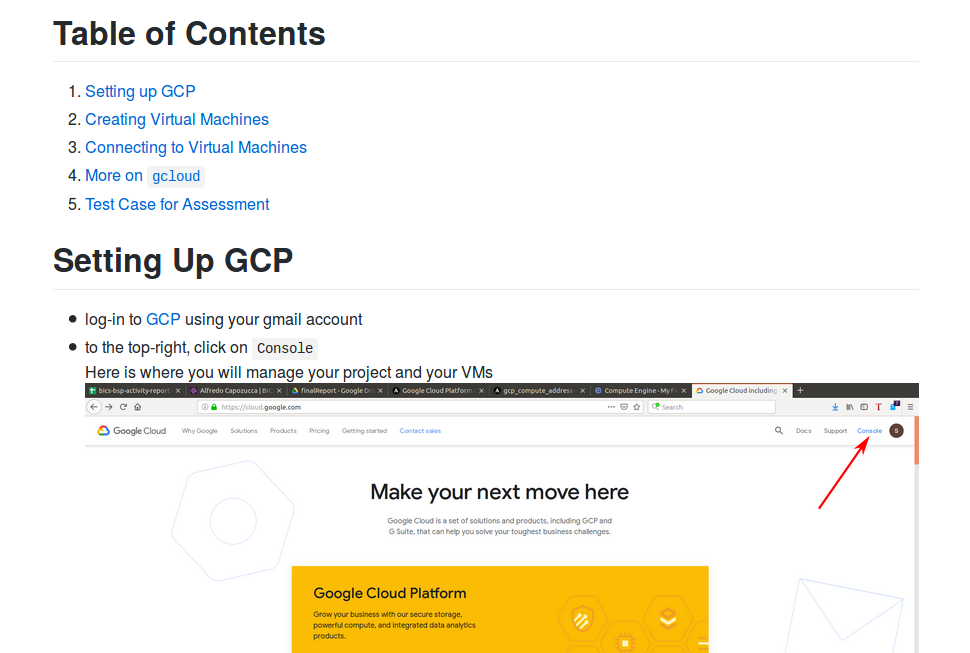
\includegraphics[width=.5\textwidth]{Images/markdown-showcase.png}
%     \caption{Markdown example}
%     \label{fig:markdown}
% \end{figure}

Here we have, for instance, the table of contents which is followed by
a few items colored in blue. This means that you can click on it to
jump some place else. For the table of content, it makes you jump to
the corresponding section in the tutorial. Also, in the first bullet
point in the figure, you can see that \textit{GCP} is colored blue.
This one will actually take you to the Google Cloud Platform.  We used
this all throughout the tutorial to send the reader, in case of need,
to a specific section to get a refresher or some additional
information.

% \subsection{Assessment ($\pm$ 15\% of section's words)}
% % Due to time constraints, we are not going to use the Excalibur
% Tutorial as our test case. Instead, we will do a few basic tasks to
% check if the machine is usable.

% We are going to download and install Remarkable for this purpose.
% Since downloading and installing software will be part of the tasks
% required to set up Excalibur, this seems like a good trade off.

% Further, to make this test case more adapted to a real life situation,
% we will be running one or two Youtube videos in the background as well
% as having a word editor opened while doing the installation.

% If we give our machine enough resources to work properly, then these
% tasks should be doable without any major problems.

We will evaluate the solution with regards to the non-functional
requirements to check how well these have been tackled. Admittedly,
the only part of the final solution that has not been solved yet is to
automatically ensure SSH and RDP\footnote{Remote Desktop Protocol is
used for sharing the Desktop of the instance} access once the instance
is created.  So this is a step which the DevOps engineer needs to do
manually before being able to respectively provision the machine and
set up the Excalibur Environment.

Also, we will consider that the DevOps engineer uses the solution
provided on GitHub more than once since the first time around there
are quite a few things to set up but after that, the deployment of new
instances is quite fast. So for the evaluation we will not consider
the things you have to do the very first time.

We will use the following scale ranging from handled the worst to
handled the best for evaluation purposes: \verb|--|, \verb|-|,
\verb|+|, \verb|++|.

\begin{enumerate}

	\item \textbf{Operability}.  In order to evaluate
	this we will take into consideration all the things the DevOps
	engineer must be able to do beforehand in order to tackle the
	given solution.

	For our solution, the DevOps engineer must at least know how to
	set up GCP and a project, how to set up the gcloud command line
	tool and how to get SSH access to the instances. After that, the
	scripts handle pretty much everything. Granted, the tutorial we
	provided gives step by step instructions for these tasks. Thus we
	conclude that the operability is \verb|+|.

	\item \textbf{Efficiency}. In order to evaluate
	this non-functional requirement, we will look at the amount of
	steps necessary to acquire the Virtual Machine and get them ready
	for the Excalibur Environment. We will orient ourselves on the
	tutorial that will be presented along side the script.

	If you want to create the virtual machine manually it will take
	you 3 steps. If you opt for the script or gcloud tool there is
	only 1 step. Although the gcloud tool might take you a few more
	steps to find the right things to put in the flags.

	For provisioning you have to set up SSH access manually and
	afterwards you need to set up RDP access as well. These two steps
	might be a little cumbersome. So the efficiency is \verb|+|.

	\item \textbf{Satisfaction}.  In order to evaluate
	this, we will again look at the amount of steps necessary but also
	at the time required to execute them.  This is due to the fact
	that more and lengthy steps to follow decrease the ease and speed
	at which you can repeat a given solution.

	We have two steps on SSH and RDP that need to be done manually and
	that may be a little annoying, but at the same time we give the
	user the possibility to use an Excalibur Environment with great
	ease. In fact, the Excalibur user does not have to do anything at
	all. Despite the two manual interactions we will say, thanks to
	the great satisfaction on the user's side, that satisfaction is
	\verb|++|.

	\item \textbf{Maintainability}.  For evaluation of this
	non-functional requirement, we look at how difficult and how much
	effort it may take for the DevOps engineer to tweak the creation
	and provisioning.

	The two steps that require manual intervention, namely the SSH and
	RDP setup, do not give rise to maintainability issues because you
	set them up once and there is nothing to worry about anymore.
	Added to the fact that everything is handled by scripts which you
	can go and edit, we conclude that maintainability is \verb|++|.

	\item \textbf{Reliability}.  For our evaluation purpose, we will
	try to look at how many things can go wrong during the Virtual
	Machine creation as well as setting up remote access. So the fewer
	things there are that can go wrong, the more reliable the solution
	will be.

	Except for the two steps in setting up SSH and RDP nothing can
	really go wrong because the script handles the rest and we are
	granted with a certain level of reliability, concerning the
	virtual machines, on GCP's part. For setting up SSH there are not
	too many things that can go wrong considering there are not a lot
	of steps and they are rather simple. However the RDP setup
	requires a few steps that may or may not demand a little more
	attention, since you need to have a look at one or the other
	configuration file.  Hence we will say that reliability is
	\verb|+|.

	\item \textbf{Adaptability}. To evaluate this non-functional
	requirement, we will consider the ease with which you can adapt an
	instance to a given situation.
	
	Due to the fact that instances are not physical, we can pretty
	easily tweak their properties. We should note that this is not as
	easily accomplished with physical machines as with virtual
	machines. Hence adaptability is \verb|++|.

	\item \textbf{Performance efficiency}. For evaluation purpose, we
	will look at how good of a performance we can achieve with a given
	set of resources.

	Thanks to the fact that we can tweak the instance's
	properties\footnote{We are assuming that the servers where our
	instances are running on have enough resources to allow us to do
	this}, like resources, we have the ability to try and fiddle
	around with the amount of resources until we find a specification
	that yields the greatest performance with the least amount of
	resources. Due to the potential fiddling, we will say that
	performance efficiency is \verb|+|.

\end{enumerate}

The summary table \ref{tab:NFR} gives an overview of this
non-functional requirement evaluation.

\begin{table}
\centering
\begin{tabular}{l | c}
		 Non-Functional Requirement & Evaluation \\\hline
		 Operability & \verb|+| \\
		 Efficiency & \verb|+| \\
		 Satisfaction & \verb|++| \\
		 Maintainability & \verb|++| \\
		 Reliability & \verb|+| \\
		 Adaptability & \verb|++| \\
		 Performance efficiency & \verb|+|
	\end{tabular}
	\caption{NFR summary table}
	\label{tab:NFR}
\end{table}



\section*{Acknowledgment}
{\color{gray}
The authors would like to thank the BiCS management and education team
for the amazing work done.
}



\section{Conclusion}
% {\color{gray}
% The conclusion goes here.
% }

I think this BSP gave me plenty of insights into cloud computing and
why it is used. It was a very interesting subject to work on and learn
about.


% An example of a floating figure using the graphicx package.
% Note that \label must occur AFTER (or within) \caption.
% For figures, \caption should occur after the \includegraphics.
% Note that IEEEtran v1.7 and later has special internal code that
% is designed to preserve the operation of \label within \caption
% even when the captionsoff option is in effect. However, because
% of issues like this, it may be the safest practice to put all your
% \label just after \caption rather than within \caption{}.
%
% Reminder: the "draftcls" or "draftclsnofoot", not "draft", class
% option should be used if it is desired that the figures are to be
% displayed while in draft mode.
%
%\begin{figure}[!t]
%\centering
%\includegraphics[width=2.5in]{myfigure}
% where an .eps filename suffix will be assumed under latex, 
% and a .pdf suffix will be assumed for pdflatex; or what has been declared
% via \DeclareGraphicsExtensions.
%\caption{Simulation results for the network.}
%\label{fig_sim}
%\end{figure}

% Note that the IEEE typically puts floats only at the top, even when this
% results in a large percentage of a column being occupied by floats.


% An example of a double column floating figure using two subfigures.
% (The subfig.sty package must be loaded for this to work.)
% The subfigure \label commands are set within each subfloat command,
% and the \label for the overall figure must come after \caption.
% \hfil is used as a separator to get equal spacing.
% Watch out that the combined width of all the subfigures on a 
% line do not exceed the text width or a line break will occur.
%
%\begin{figure*}[!t]
%\centering
%\subfloat[Case I]{\includegraphics[width=2.5in]{box}%
%\label{fig_first_case}}
%\hfil
%\subfloat[Case II]{\includegraphics[width=2.5in]{box}%
%\label{fig_second_case}}
%\caption{Simulation results for the network.}
%\label{fig_sim}
%\end{figure*}
%
% Note that often IEEE papers with subfigures do not employ subfigure
% captions (using the optional argument to \subfloat[]), but instead will
% reference/describe all of them (a), (b), etc., within the main caption.
% Be aware that for subfig.sty to generate the (a), (b), etc., subfigure
% labels, the optional argument to \subfloat must be present. If a
% subcaption is not desired, just leave its contents blank,
% e.g., \subfloat[].


% An example of a floating table. Note that, for IEEE style tables, the
% \caption command should come BEFORE the table and, given that table
% captions serve much like titles, are usually capitalized except for words
% such as a, an, and, as, at, but, by, for, in, nor, of, on, or, the, to
% and up, which are usually not capitalized unless they are the first or
% last word of the caption. Table text will default to \footnotesize as
% the IEEE normally uses this smaller font for tables.
% The \label must come after \caption as always.
%
%\begin{table}[!t]
%% increase table row spacing, adjust to taste
%\renewcommand{\arraystretch}{1.3}
% if using array.sty, it might be a good idea to tweak the value of
% \extrarowheight as needed to properly center the text within the cells
%\caption{An Example of a Table}
%\label{table_example}
%\centering
%% Some packages, such as MDW tools, offer better commands for making tables
%% than the plain LaTeX2e tabular which is used here.
%\begin{tabular}{|c||c|}
%\hline
%One & Two\\
%\hline
%Three & Four\\
%\hline
%\end{tabular}
%\end{table}


% Note that the IEEE does not put floats in the very first column
% - or typically anywhere on the first page for that matter. Also,
% in-text middle ("here") positioning is typically not used, but it
% is allowed and encouraged for Computer Society conferences (but
% not Computer Society journals). Most IEEE journals/conferences use
% top floats exclusively. 
% Note that, LaTeX2e, unlike IEEE journals/conferences, places
% footnotes above bottom floats. This can be corrected via the
% \fnbelowfloat command of the stfloats package.

% trigger a \newpage just before the given reference
% number - used to balance the columns on the last page
% adjust value as needed - may need to be readjusted if
% the document is modified later
%\IEEEtriggeratref{8}
% The "triggered" command can be changed if desired:
%\IEEEtriggercmd{\enlargethispage{-5in}}

% references section

% can use a bibliography generated by BibTeX as a .bbl file
% BibTeX documentation can be easily obtained at:
% http://mirror.ctan.org/biblio/bibtex/contrib/doc/
% The IEEEtran BibTeX style support page is at:
% http://www.michaelshell.org/tex/ieeetran/bibtex/
%\bibliographystyle{IEEEtran}
% argument is your BibTeX string definitions and bibliography database(s)
%\bibliography{IEEEabrv,../bib/paper}
%
% <OR> manually copy in the resultant .bbl file
% set second argument of \begin to the number of references
% (used to reserve space for the reference number labels box)
\begin{thebibliography}{1}
\bibitem[BiCS(2018a)]{bics-bsp-report-template}
\newblock {BiCS Bachelor Semester Project Report Template}.
\newblock {https://github.com/nicolasguelfi/lu.uni.course.bics.global}
\newblock {University of Luxembourg, BiCS - Bachelor in Computer Science (2017).}

%\bibitem[BiCS(2018b)] {bics-bsp-reference-document}
%{Bachelor in Computer Science}:
%\newblock {BiCS Semester Projects Reference Document}.
%\newblock Technical report, University of Luxembourg (2018)
%
%\bibitem[Armstrong and Green(2017)]{armstrong2017guidelinesforscience}
%J~Scott Armstrong and Kesten~C Green.
%\newblock Guidelines for science: Evidence and checklists.
%\newblock \emph{Scholarly Commons}, pages 1--24, 2017.
%\newblock {https://repository.upenn.edu/marketing_papers/181/}

\end{thebibliography}

\newpage 
\section{Appendix}
The final solution along with the tutorial as well as this report are
on github: \url{https://github.com/niveK77pur/ExcaliburEnvironmentGCP}

\end{document}


